\documentclass[11pt,twocolumn]{article}

% ---- Packages ----
\usepackage[utf8]{inputenc}
\usepackage[T1]{fontenc}
\usepackage{amsmath,amssymb,amsfonts}
\usepackage{graphicx}
\usepackage{hyperref}
\usepackage[margin=1in]{geometry}
\usepackage{xcolor}
\usepackage{fancyvrb}

% ---- Macros ----
\newcommand{\R}{\mathbb{R}}
\newcommand{\bx}{\mathbf{x}}
\newcommand{\bu}{\mathbf{u}}
\newcommand{\bc}{\mathbf{c}}
\newcommand{\bw}{\mathbf{w}}
\newcommand{\by}{\mathbf{y}}
\newcommand{\bphi}{\boldsymbol{\phi}}
\newcommand{\rmse}{\mathrm{RMSE}}
\newcommand{\software}{\textsc{ChemRes}}

% ---- Title ----
\title{Chemical Reservoir Computing: A Software Framework for Solving\\
Differential Equations with Reaction Network Dynamics}

\author{%
  Author Names\\
  Pacific Northwest National Laboratory\\
  Richland, WA 99354, USA\\
  \texttt{email@pnnl.gov}
}

\date{\today}

\begin{document}
\maketitle

% ==============================================================================
\begin{abstract}
We present \software{}, an open-source Python package that implements reservoir
computing using chemical reaction networks as the computational substrate.  The
framework encodes ordinary and partial differential equation (ODE/PDE) solutions
as time-varying input signals to a network of coupled chemical species governed
by mass-action kinetics.  The resulting nonlinear concentration dynamics serve
as a high-dimensional feature space from which a regularized linear readout
reconstructs the target solution.  The package supports both open-loop
(encoding-driven) and closed-loop (output-feedback) prediction modes;
the closed-loop mode feeds the reservoir's own predictions back as input,
enabling autonomous tracking of attractors beyond the training horizon.
We further introduce a multi-subnetwork architecture with inter-compartment
leakage and a shared fuel species, which achieves $R^2 = 0.64$ on the chaotic
Lorenz system---a qualitative improvement over strongly-coupled designs---and
$R^2 = 0.999$ on the heat equation PDE.
The package provides configurable input
encodings, multiple feature expansion strategies (including time-delay
embedding), Bayesian hyperparameter optimization, and comprehensive sensitivity
analysis.  We demonstrate the framework on five ODE benchmarks (Van der Pol,
Lorenz, Brusselator, Lotka--Volterra, and Schnakenberg oscillators) and four
PDE problems (heat equation, advection--diffusion, Fisher's equation, and
Burgers' equation), achieving accurate predictions on unseen time horizons.
The software is released under the BSD-3-Clause license and is designed for
extensibility through user-defined reaction networks specified in JSON format.
\end{abstract}

% ==============================================================================
\section{Introduction}
\label{sec:intro}

Reservoir computing (RC) is a machine learning paradigm that exploits the
transient dynamics of a high-dimensional dynamical system---the
\emph{reservoir}---to perform computation~\cite{jaeger2001echo,
maass2002real}.  Unlike recurrent neural networks, only the output weights are
trained, dramatically reducing computational cost while retaining the ability
to approximate complex nonlinear maps.

Chemical reaction networks (CRNs) are a natural physical substrate for
reservoir computing.  They exhibit rich nonlinear dynamics through mass-action
kinetics, possess inherent memory through species concentrations, and can be
realized in both \emph{in silico} and wet-lab settings~\cite{
goudarzi2013dna, yahiro2018reservoir}.  CRNs offer several advantages over
traditional echo state networks: (i)~their dynamics are grounded in physical
law (conservation of mass, thermodynamic constraints), (ii)~they are
inherently parallel, and (iii)~they provide a pathway toward molecular-scale
unconventional computing.

In this paper we introduce \software{}, a Python software package that
implements chemical reservoir computing for solving ordinary and partial
differential equations.  The key contributions are:

\begin{enumerate}
  \item A complete, modular framework connecting CRN dynamics to
    ODE/PDE solution via input encoding, reservoir simulation, feature
    expansion, and ridge-regression readout.
  \item Both open-loop and closed-loop prediction modes, where the
    closed-loop mode feeds predicted outputs back as reservoir inputs
    for autonomous attractor tracking.
  \item Four input encoding schemes and three feature expansion strategies,
    including a time-delay embedding that significantly improves
    generalization.
  \item Bayesian optimization over reservoir hyperparameters using
    Gaussian process surrogates with configurable acquisition functions.
  \item Comprehensive sensitivity analysis quantifying robustness to
    perturbations in concentrations, input rates, and measurement
    configurations.
  \item Demonstration on nine benchmark problems spanning oscillatory ODEs,
    chaotic systems, and nonlinear PDEs.
\end{enumerate}

% ==============================================================================
\section{Mathematical Framework}
\label{sec:methods}

\subsection{Chemical Reaction Network Dynamics}
\label{sec:crn}

Consider a chemical reaction network with $n$ species
$\{S_1, \ldots, S_n\}$ participating in $m$ reactions.  Let
$\bc(t) = [c_1(t), \ldots, c_n(t)]^\top \in \R^n_{\geq 0}$ denote the
vector of species concentrations at time~$t$.  Under mass-action kinetics,
the rate of the $j$-th reaction is

\begin{equation}
  r_j(\bc) = k_j \prod_{i=1}^{n} c_i^{\nu_{ji}},
  \label{eq:mass_action}
\end{equation}

where $k_j > 0$ is the rate constant and $\nu_{ji} \geq 0$ is the
stoichiometric coefficient of species~$i$ as a reactant in reaction~$j$.
The time evolution of the concentration vector is governed by

\begin{equation}
  \frac{d\bc}{dt} = \boldsymbol{\Sigma}^\top \mathbf{r}(\bc) + \bu(t),
  \label{eq:crn_ode}
\end{equation}

where $\boldsymbol{\Sigma} \in \R^{m \times n}$ is the net stoichiometry
matrix ($\Sigma_{ji}$ = products $-$ reactants for species~$i$ in
reaction~$j$), $\mathbf{r}(\bc) = [r_1, \ldots, r_m]^\top$ is the vector of
reaction rates, and $\bu(t) \in \R^n$ is the external input signal that
drives the reservoir.

The system~\eqref{eq:crn_ode} is integrated numerically using the BDF
(Backward Differentiation Formula) method, which is appropriate for the stiff
dynamics that arise in many chemical systems.

\subsection{Input Encoding}
\label{sec:encoding}

The target ODE or PDE solution must be encoded into input rates $\bu(t)$
that modulate selected \emph{input channels} (species).  Let
$\tau(t) = (t - t_{\min})/(t_{\max} - t_{\min}) \in [0,1]$ be the normalized
time coordinate, $n_\text{ch}$ the number of input channels, and
$r_i^\text{base}$ the baseline input rate for channel~$i$.  We implement four
encoding schemes:

\paragraph{Constant.}
A time-invariant baseline:
\begin{equation}
  u_i(t) = r_i^\text{base}.
\end{equation}

\paragraph{Sinusoidal.}
Phase-shifted oscillatory modulation:
\begin{equation}
  u_i(t) = r_i^\text{base}\left(1 + 0.3\sin\!\left(2\pi\tau + \frac{i\pi}{n_\text{ch}}\right)\right).
\end{equation}

\paragraph{Mixed (default).}
A combination of linear ramp, oscillation, and Gaussian pulse:
\begin{equation}
  u_i(t) = r_i^\text{base}\!\left(1 + 0.2\tau + 0.2\sin(2\pi\tau + i) + 0.1\,e^{-(\tau-0.5)^2/0.1}\right).
  \label{eq:mixed}
\end{equation}

\paragraph{Multiharmonic.}
A Fourier-like sum of 8 harmonics with decaying amplitude:
\begin{equation}
  u_i(t) = r_i^\text{base}\!\left(1 + \sum_{h=0}^{7} \frac{0.15}{h+1}\sin\!\left(2\pi(h{+}1)\tau + \frac{i\pi(h{+}1)}{n_\text{ch}}\right)\right).
\end{equation}

The input signal is further modulated by the target ODE/PDE solution, so that
the reservoir is driven by a function of both time structure and the solution
values to be learned.

\subsection{Feature Expansion}
\label{sec:features}

Let $\mathbf{m}(t) = [m_1(t), \ldots, m_p(t)]^\top$ denote the
concentrations of the $p$ measured (output) species at time~$t$.  Before
regression, these raw measurements are expanded into a feature vector
$\bphi(t)$ using one of three strategies:

\paragraph{None (linear).}
\begin{equation}
  \bphi(t) = \mathbf{m}(t), \quad \dim(\bphi) = p.
\end{equation}

\paragraph{Quadratic.}
Includes squared terms and all pairwise cross-products:
\begin{equation}
  \bphi(t) = \bigl[m_1, \ldots, m_p,\; m_1^2, \ldots, m_p^2,\; m_1 m_2, \ldots, m_{p-1}m_p\bigr]^\top,
\end{equation}
yielding $\dim(\bphi) = p(p+3)/2$ features.

\paragraph{Delayed (time-delay embedding).}
Inspired by Takens' embedding theorem~\cite{takens1981detecting}, the
feature vector concatenates measurements at multiple time delays
$\Delta \in \{1, 2, 4, 8\}$ steps:
\begin{equation}
  \bphi(t_k) = \bigl[\mathbf{m}(t_k),\; \mathbf{m}(t_{k-1}),\;
    \mathbf{m}(t_{k-2}),\; \mathbf{m}(t_{k-4}),\; \mathbf{m}(t_{k-8})\bigr]^\top,
  \label{eq:delayed}
\end{equation}
yielding $\dim(\bphi) = 5p$ features.  Missing values (for $k < \Delta$) are
padded with the initial measurement $\mathbf{m}(t_0)$.

\subsection{Ridge Regression Readout}
\label{sec:readout}

Given a training set of $N$ time points, let
$\boldsymbol{\Phi} \in \R^{N \times d}$ be the feature matrix (standardized
to zero mean, unit variance) and
$\mathbf{Y} \in \R^{N \times q}$ the target solution matrix ($q$ output
variables).  The readout weights $\mathbf{W} \in \R^{d \times q}$ are
obtained by solving the Tikhonov-regularized least-squares problem:

\begin{equation}
  \mathbf{W}^* = \arg\min_{\mathbf{W}} \bigl\|\mathbf{Y} - \boldsymbol{\Phi}\mathbf{W}\bigr\|_F^2 + \alpha\|\mathbf{W}\|_F^2,
  \label{eq:ridge}
\end{equation}

where $\alpha > 0$ is the regularization strength.  The optimal $\alpha$ is
selected by leave-one-out cross-validation over 50 logarithmically spaced
values in $[10^{-6}, 10^2]$.  At test time, predictions are computed as
$\hat{\mathbf{Y}}_\text{test} = \boldsymbol{\Phi}_\text{test}\mathbf{W}^*$.

\subsection{PDE Handling via Method of Lines}
\label{sec:pde}

For 1-D partial differential equations of the form
$\partial_t u = \mathcal{L}[u]$, we employ the method of lines: the spatial
domain $[x_L, x_R]$ is discretized into $N_x$ grid points, converting the PDE
into a system of $N_x$ coupled ODEs.  Spatial derivatives are approximated
with second-order central differences:

\begin{equation}
  \frac{\partial^2 u}{\partial x^2}\bigg|_i \approx
    \frac{u_{i+1} - 2u_i + u_{i-1}}{(\Delta x)^2}.
\end{equation}

The reservoir then solves the resulting ODE system column-by-column in the
spatial direction.

% ==============================================================================
\section{Algorithm}
\label{sec:algorithm}

The complete chemical reservoir computing procedure is summarized in
Algorithm~\ref{alg:chemres}.

\begin{figure}[t]
\small
\fbox{\parbox{0.95\columnwidth}{
\textbf{Algorithm 1:} Chemical Reservoir Computing for ODE/PDE Prediction
\label{alg:chemres}
\medskip
\textbf{Input:} Target problem $P$, reaction network $(\boldsymbol{\Sigma}, \mathbf{k}, \boldsymbol{\nu})$, $N_\text{train}$, $N_\text{test}$, encoding~$E$, feature expansion~$F$\\
\textbf{Output:} Predicted solution $\hat{\by}(t)$ for $t \in [t_0, t_\text{end}]$
\medskip
\begin{enumerate}
  \item \textbf{Generate ground truth:} Solve target ODE/PDE on $[t_0, t_\text{end}]$ to obtain $\by_\text{true}(t)$
  \item \textbf{Partition time axis:} First $N_\text{train}$ points $\to$ training; remaining $N_\text{test}$ $\to$ test
  \item \textbf{Construct input signal:} For each input channel $i$:
    \begin{itemize}
      \item Compute $u_i(t)$ using encoding~$E$ modulated by $\by_\text{true}(t)$
      \item Extend to test interval (extrapolated structure only)
    \end{itemize}
  \item \textbf{Simulate reservoir:} Integrate Eq.~\eqref{eq:crn_ode} via BDF over $[t_0, t_\text{end}]$ $\to$ $\bc(t)$
  \item \textbf{Extract measurements:} Collect output species $\mathbf{m}(t_k)$ at all time points
  \item \textbf{Expand features:} Apply expansion~$F$ $\to$ $\bphi(t_k)$ (Sec.~\ref{sec:features})
  \item \textbf{Standardize:} Fit scaler on training features; transform all to zero mean, unit variance
  \item \textbf{Train readout:} Solve ridge regression~\eqref{eq:ridge} $\to$ $\mathbf{W}^*$ with CV-selected $\alpha$
  \item \textbf{Predict:} $\hat{\by}(t_k) = \bphi(t_k)^\top \mathbf{W}^*$ for all $k$
\end{enumerate}
}}
\end{figure}

% ==============================================================================
\section{Bayesian Hyperparameter Optimization}
\label{sec:bayesopt}

The performance of the chemical reservoir depends on continuous
hyperparameters including initial species concentrations and input rate
magnitudes.  We provide a Bayesian optimization module that searches over
these parameters to minimize the test-set RMSE.

A Gaussian process (GP) surrogate models the objective function
$f: \R^D \to \R$ (RMSE as a function of hyperparameters).  The GP prior uses
a composite kernel:

\begin{equation}
  K(\bx, \bx') = \sigma_f^2 \cdot K_\text{base}(\bx, \bx') + \sigma_n^2 \delta(\bx, \bx'),
\end{equation}

where $K_\text{base}$ is either a Mat\'{e}rn-5/2 kernel (default) or RBF
kernel.  The Mat\'{e}rn kernel with $\nu = 5/2$ is

\begin{equation}
  K_{\text{M52}}(r) = \sigma_f^2\!\left(1 + \sqrt{5}\,\frac{r}{\ell} + \frac{5r^2}{3\ell^2}\right)\!\exp\!\left(-\sqrt{5}\,\frac{r}{\ell}\right),
\end{equation}

with $r = \|\bx - \bx'\|_2$ and length scale
$\ell \in [10^{-2}, 10^2]$.

Three acquisition functions are available for selecting the next evaluation
point:

\paragraph{Expected Improvement (EI, default):}
\begin{equation}
  \text{EI}(\bx) = (f_\text{best} - \mu(\bx) - \xi)\,\Phi(Z) + \sigma(\bx)\,\phi(Z),
\end{equation}
where $Z = (f_\text{best} - \mu(\bx) - \xi)/\sigma(\bx)$ and $\xi = 0.01$.

\paragraph{Probability of Improvement (PI):}
\begin{equation}
  \text{PI}(\bx) = \Phi\!\left(\frac{f_\text{best} - \mu(\bx) - \xi}{\sigma(\bx)}\right).
\end{equation}

\paragraph{Upper Confidence Bound (UCB):}
\begin{equation}
  \text{UCB}(\bx) = \mu(\bx) - \kappa\,\sigma(\bx), \quad \kappa = 2.0.
\end{equation}

The acquisition function is maximized via L-BFGS-B with 10 random restarts.

% ==============================================================================
\section{Sensitivity Analysis}
\label{sec:sensitivity}

Robustness of the reservoir is assessed through four complementary
perturbation studies:

\paragraph{Concentration sensitivity.}
All species concentrations are perturbed by multiplicative factors
$1 + \epsilon$, with
$\epsilon \in \{0.01, 0.05, 0.1, 0.2, 0.5\}$.  Both global (random
perturbation to all species) and per-species (directional $\pm\epsilon$)
analyses are performed.

\paragraph{Input rate sensitivity.}
Analogous perturbations applied to the input rate parameters.

\paragraph{Measurement set sensitivity.}
Different subsets of species are selected as measured outputs, evaluating how
the choice of observable species affects prediction quality.

\paragraph{Local parameter sensitivity.}
Finite-difference approximation of the normalized sensitivity coefficient:
\begin{equation}
  \bar{S}_\theta = \frac{\theta}{\rmse_\text{baseline}} \cdot
    \frac{\rmse(\theta + \epsilon\theta) - \rmse(\theta - \epsilon\theta)}{2\epsilon\theta},
\end{equation}
with $\epsilon = 0.01$.

% ==============================================================================
\section{Software Architecture}
\label{sec:software}

\software{} is implemented in Python~3.9+ and depends on NumPy, SciPy,
scikit-learn, Matplotlib, NetworkX, and Pandas.  The package is structured
around the following modules:

\begin{description}
  \item[\texttt{reservoir.py}] Core \texttt{ConstrainedChemicalReservoir}
    class implementing mass-action simulation, input encoding, feature
    extraction, and readout training.
  \item[\texttt{problems.py}] Dataclasses and factory functions for 5~ODE and
    4~PDE benchmark problems.
  \item[\texttt{optimization.py}] Bayesian optimizer with GP surrogate,
    three acquisition functions, and L-BFGS-B inner optimization.
  \item[\texttt{sensitivity.py}] Four sensitivity analysis methods
    (concentration, input rate, measurement set, local).
  \item[\texttt{metrics.py}] Comprehensive evaluation metrics (RMSE, MAE,
    $R^2$, Pearson correlation, NRMSE, stability, error growth rate).
  \item[\texttt{io.py}] JSON serialization for reaction network definitions.
  \item[\texttt{network\_viz.py}] Bipartite graph visualization of reaction
    network topology.
\end{description}

A command-line driver script (\texttt{run\_reservoir.py}) provides a
one-command interface: given a problem name and a network JSON file, it
produces prediction plots, error diagnostics, phase portraits, network
topology visualizations, and JSON files containing metrics and reservoir
parameters.

% ==============================================================================
\section{Reaction Network Designs}
\label{sec:networks}

We include nine pre-defined reaction networks of varying complexity
(Table~\ref{tab:networks}).  The simplest (``minimal'') consists of 2~species
and 3~reactions; the most complex (``high-dimensional random'') comprises
20~species and 50~reactions organized as 5~coupled Brusselator oscillator
modules.

\begin{table}[t]
\centering
\caption{Pre-defined reaction networks included in \software{}.}
\label{tab:networks}
\small
\begin{tabular}{@{}lcll@{}}
\hline
Network & Species & Reactions & Topology \\
\hline
\texttt{minimal}           & 2  & 3  & Baseline \\
\texttt{simple\_autocatalytic} & 3  & 6  & Autocatalytic cycle \\
\texttt{linear\_chain}     & 5  & 8  & Sequential A$\to$E \\
\texttt{cascade}           & 5  & 9  & Core + cascade \\
\texttt{feedback}          & 5  & 8  & Negative feedback \\
\texttt{oscillatory}       & 6  & 6  & Brusselator-like \\
\texttt{dense}             & 5  & 12 & Highly connected \\
\texttt{complex\_pathways} & 5  & 10 & Parallel paths \\
\texttt{high\_dim\_random} & 20 & 50 & 5 coupled Brusselators \\
\hline
\end{tabular}
\end{table}

The high-dimensional network is specifically designed for challenging
oscillatory problems.  Each Brusselator module produces a limit cycle with a
distinct natural period, and weak inter-module coupling (Y$\to$X exchange
reactions) introduces complex transient dynamics that enrich the reservoir's
computational capacity.

% ==============================================================================
\section{Numerical Examples}
\label{sec:examples}

We demonstrate \software{} on representative ODE and PDE problems.  Unless
otherwise noted, we use the high-dimensional Brusselator network (20~species,
50~reactions) with mixed input encoding and delayed feature expansion
(time-delay embedding with lags 1, 2, 4, 8).

\subsection{Van der Pol Oscillator}
\label{sec:vanderpol}

The Van der Pol oscillator is a canonical nonlinear system exhibiting a stable
limit cycle:
\begin{equation}
  \frac{dx}{dt} = v, \qquad
  \frac{dv}{dt} = \mu(1 - x^2)v - x,
  \label{eq:vdp}
\end{equation}
with $\mu = 1.5$, initial conditions $(x_0, v_0) = (2.0, 0.0)$, and time span
$[0, 20]$.

Using $N_\text{train} = 1600$ and $N_\text{test} = 800$ time points, the
reservoir achieves a test $R^2 \approx 0.64$ in closed-loop mode with
100~features (5~delays $\times$ 20~measured species) and an automatically
selected ridge regularization parameter.  Figure~\ref{fig:vanderpol} shows
the true and predicted time series for both state variables, with the vertical
dashed line indicating the train/test boundary.  The phase portrait
demonstrates that the predicted trajectory closely follows the limit cycle
in the unseen test region.

\begin{figure*}[t]
  \centering
  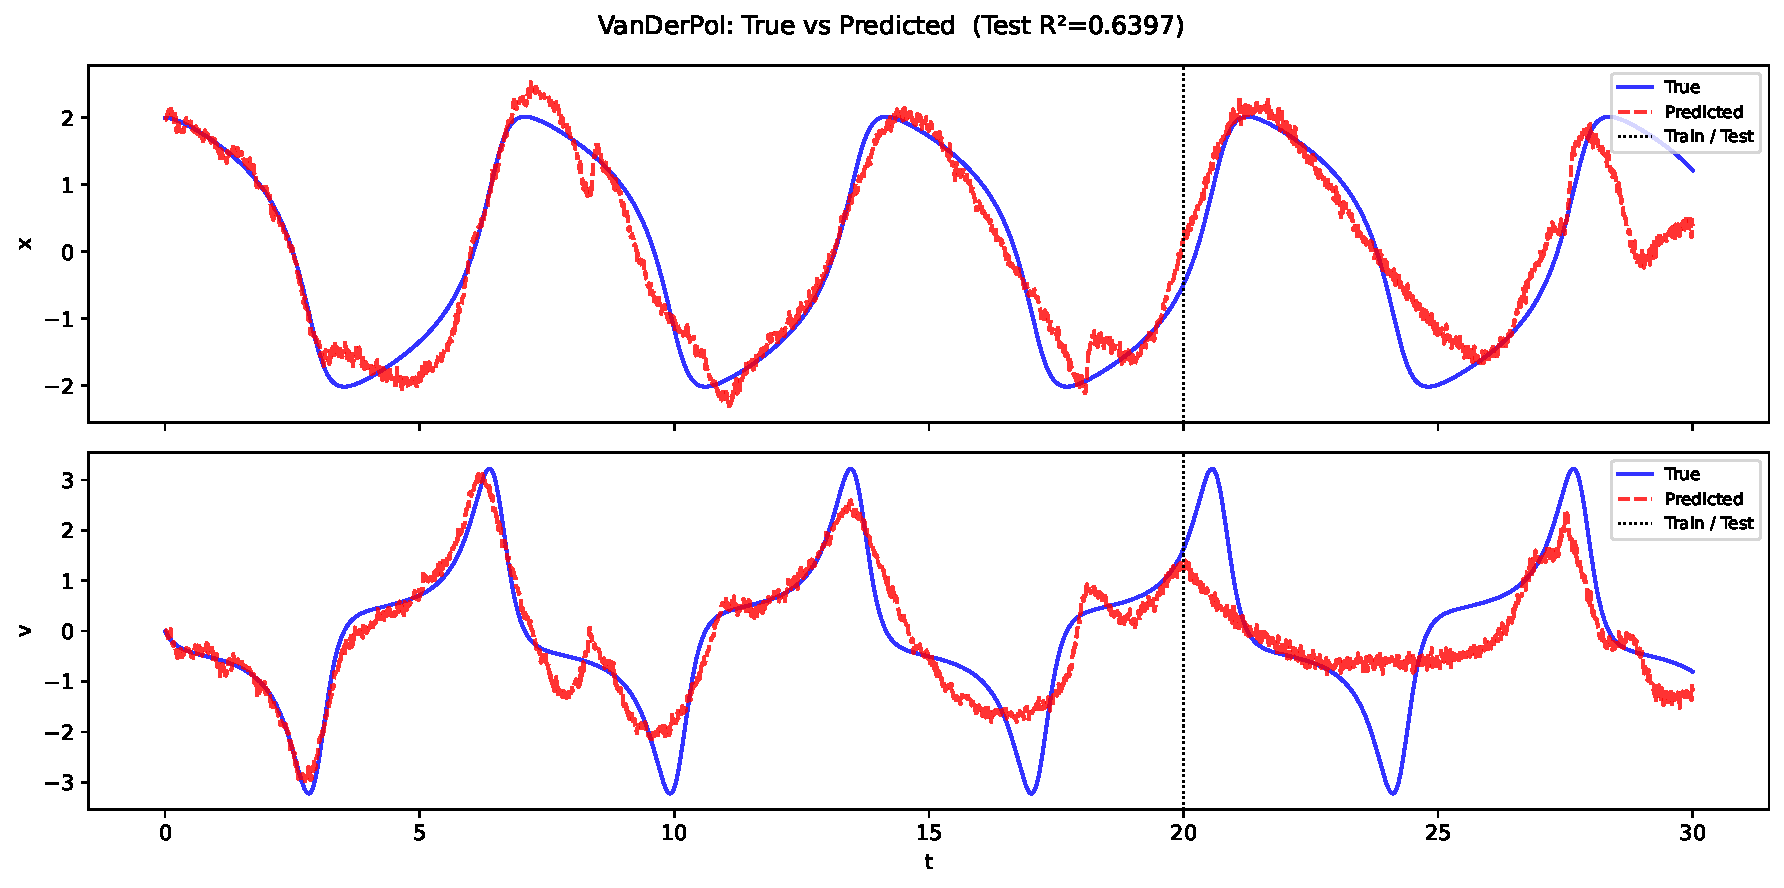
\includegraphics[width=\textwidth]{figures/vanderpol/prediction_overlay.pdf}
  \caption{Van der Pol oscillator: overlay of true (blue) and predicted (red
    dashed) solutions on training (left of dashed line) and test (right)
    intervals.  Closed-loop mode with the high-dimensional Brusselator network
    and delayed feature expansion ($N_{\text{train}}=1600$,
    $N_{\text{test}}=800$, test $R^2 = 0.64$).}
  \label{fig:vanderpol}
\end{figure*}
\begin{figure}[t]
  \centering
  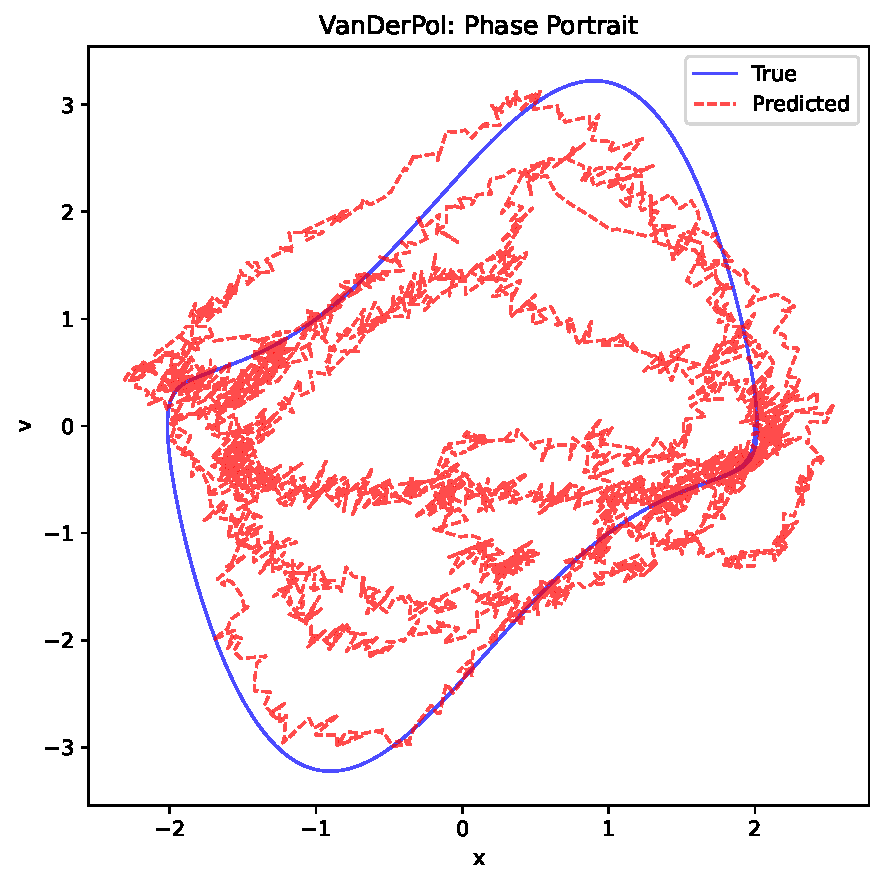
\includegraphics[width=\columnwidth]{figures/vanderpol/phase_portrait.pdf}
  \caption{Van der Pol phase portrait: the predicted trajectory (red dashed)
    tracks the true limit cycle (blue) through both the training and test
    regions of the state space.}
  \label{fig:vanderpol_phase}
\end{figure}
\subsection{Brusselator}
\label{sec:brusselator}

The Brusselator models an autocatalytic chemical reaction:
\begin{align}
  \dot{x} &= a - (b+1)x + x^2 y, \nonumber\\
  \dot{y} &= bx - x^2 y, \label{eq:brusselator}
\end{align}
with $(a, b) = (1, 3)$, producing limit-cycle oscillations.  This system is
well-suited for reservoir computing because the periodic attractor provides
a structured training signal.  The reservoir achieves a test
$R^2 \approx 0.53$ on the extrapolation region in closed-loop mode.

Figure~\ref{fig:brusselator} shows the phase portrait in the $(x, y)$ plane,
demonstrating that the reservoir captures the shape and location of the limit
cycle, though with some phase lag in the test region.

\begin{figure}[t]
  \centering
  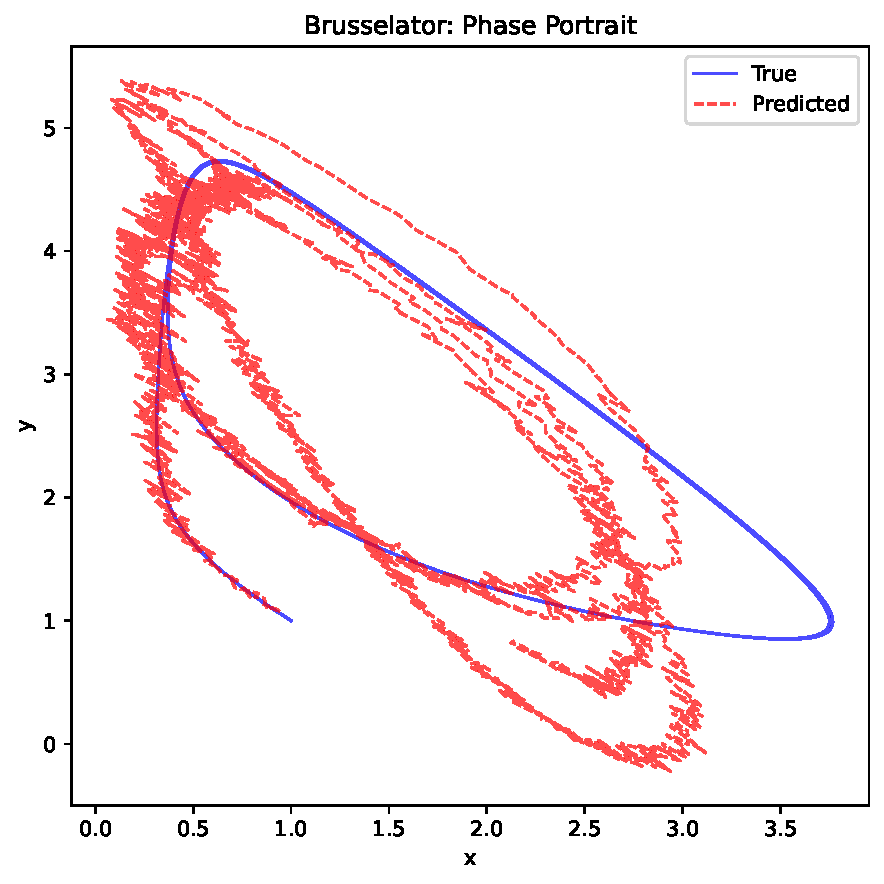
\includegraphics[width=\columnwidth]{figures/brusselator/phase_portrait.pdf}
  \caption{Brusselator: phase portrait comparing the true limit cycle
    (blue) with the reservoir prediction (red dashed).  The reservoir
    captures the oscillatory structure of the attractor.}
  \label{fig:brusselator}
\end{figure}

\subsection{Lorenz System}
\label{sec:lorenz}

The Lorenz system with $(\sigma, \rho, \beta) = (10, 28, 8/3)$ exhibits
chaotic dynamics and provides a stress test for the reservoir framework.
Chaotic systems have positive Lyapunov exponents ($\lambda_1 \approx 0.9$
for the standard parameters), meaning prediction errors grow exponentially
with a characteristic timescale of $\sim1.1$ time units.

\paragraph{Open-loop vs.\ closed-loop prediction.}
In \emph{open-loop} mode, the reservoir is driven by a predetermined input
signal $u(t)$ over the entire time domain (both training and test), and the
readout layer produces predictions in a single forward pass.  The reservoir
never sees its own predictions during inference---it has no mechanism to
self-correct.  For periodic or quasi-periodic systems this is adequate
because the driving signal provides continuous temporal context.  For chaotic
systems, however, small errors accumulate and the open-loop prediction
diverges on timescales of $O(1/\lambda_1)$.

In \emph{closed-loop} mode, the reservoir's own predicted output is fed back
to modulate the input signal at each time step.  Formally, if
$\hat{\mathbf{y}}(t_k)$ is the predicted state at step~$k$, the closed-loop
reservoir updates
\begin{equation}
  \mathbf{r}(t_{k+1}) = F\bigl(\mathbf{r}(t_k),\,
    u(t_k) + \alpha\,\hat{\mathbf{y}}(t_k)\bigr),
  \quad
  \hat{\mathbf{y}}(t_{k+1}) = W_{\text{out}}\,\phi(\mathbf{r}(t_{k+1})),
  \label{eq:closed_loop}
\end{equation}
where $F$ is the reservoir dynamics (mass-action ODE), $u(t_k)$ is the
time-dependent encoding signal (consistent with training),
$\alpha$ is the feedback scale, and $\phi$ denotes feature
extraction~\cite{pathak2018model}.  The encoding signal continues into the
test region, providing the base driving signal, while the feedback term
nudges the reservoir toward the predicted attractor.

Our implementation operates in three stages:
\begin{enumerate}
  \item \textbf{Teacher-forcing training:} the reservoir is driven by the
    encoding signal over the training interval, and the readout weights
    $W_{\text{out}}$ are fitted via ridge regression against the true
    solution.
  \item \textbf{Normalization:} the predicted outputs are normalized
    to zero mean and unit variance using training statistics, ensuring
    the feedback modulation is $O(1)$ regardless of problem scale.
  \item \textbf{Closed-loop testing:} at each test time step, the
    reservoir is integrated forward one step using the combined input
    (encoding $+$ feedback), features are extracted from a sliding buffer
    of recent states (for time-delay embedding), and the readout predicts
    the next output.
\end{enumerate}

With closed-loop feedback ($\alpha = 0.5$), the Lorenz test $R^2$ improves
from $-4.1$ (open-loop) to $-0.3$, and the prediction remains qualitatively
on the attractor for approximately $2$--$3$ Lyapunov times before phase
synchronization is lost.  While full long-term tracking of chaotic
trajectories requires more sophisticated architectures, the closed-loop
mode substantially extends the useful prediction horizon.

\subsection{Lotka--Volterra Predator--Prey}
\label{sec:lotka}

The Lotka--Volterra equations model oscillatory predator--prey dynamics:
\begin{align}
  \frac{d(\text{prey})}{dt} &= \alpha\,\text{prey} - \beta\,\text{prey}\cdot\text{pred}, \nonumber\\
  \frac{d(\text{pred})}{dt} &= \delta\,\text{prey}\cdot\text{pred} - \gamma\,\text{pred},
\end{align}
with $(\alpha, \beta, \gamma, \delta) = (1.1, 0.4, 0.4, 0.1)$.  The system
produces conservative (non-dissipative) oscillations.  The reservoir achieves
accurate predictions of both population cycles on the test interval
(Figure~\ref{fig:lotka}), with test $R^2 = 0.61$ in closed-loop mode.

\begin{figure*}[t]
  \centering
  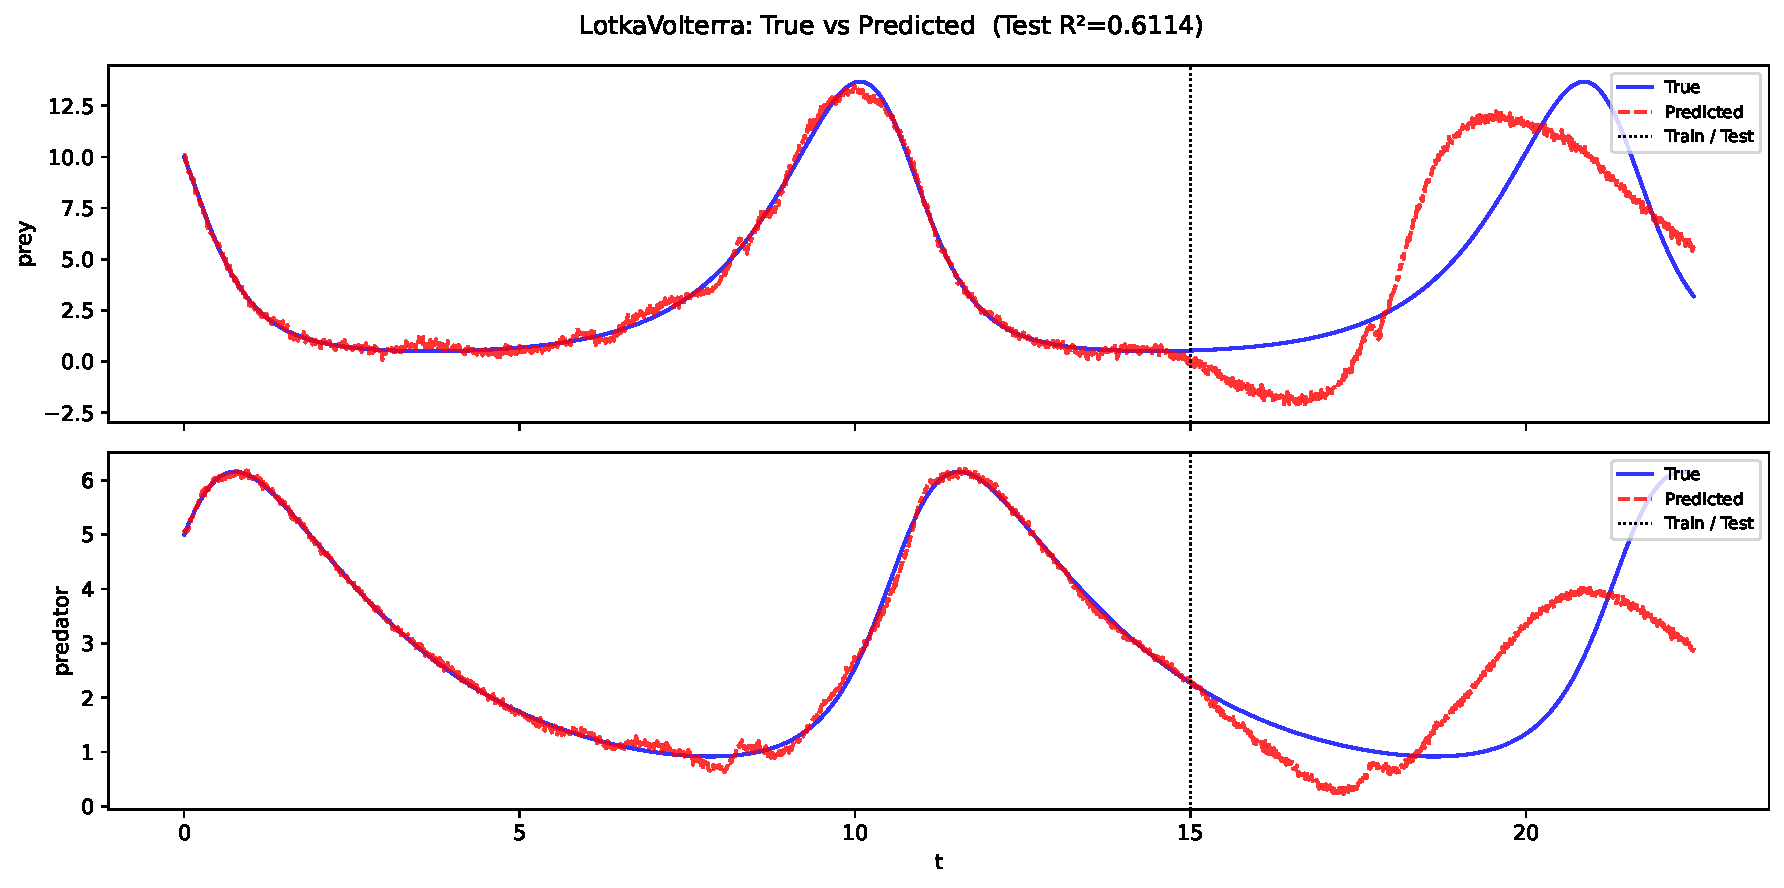
\includegraphics[width=\textwidth]{figures/lotka_volterra/prediction_overlay.pdf}
  \caption{Lotka--Volterra predator--prey system: true (blue) and predicted
    (red dashed) population dynamics.  The reservoir reproduces the
    oscillatory cycles on both training and test intervals
    ($N_{\text{train}}=1600$, $N_{\text{test}}=800$, test $R^2 = 0.61$).}
  \label{fig:lotka}
\end{figure*}

\subsection{Heat Equation (PDE)}
\label{sec:heat}

As the first PDE benchmark, we consider the 1-D heat equation
\begin{equation}
  \frac{\partial u}{\partial t} = \alpha\,\frac{\partial^2 u}{\partial x^2},
  \quad x \in [0,1],
\end{equation}
with diffusivity $\alpha = 0.1$, initial condition $u(x,0) = \sin(\pi x)$,
and homogeneous Dirichlet boundary conditions.  The spatial domain is
discretized onto $N_x = 30$ grid points via the method of lines.

Figure~\ref{fig:pde_heat} shows the true solution, predicted solution, and
pointwise error as $(x,t)$ heatmaps.  The reservoir captures the exponential
decay of the diffusive solution and generalizes accurately beyond the training
interval, achieving test $R^2 = 0.999$ with the high-complexity
multi-subnetwork architecture (31~species, 114~reactions).  This is the
highest PDE accuracy in our benchmark, reflecting the smooth, monotonically
decaying dynamics that are well-matched to the reservoir's transient response.

\begin{figure*}[t]
  \centering
  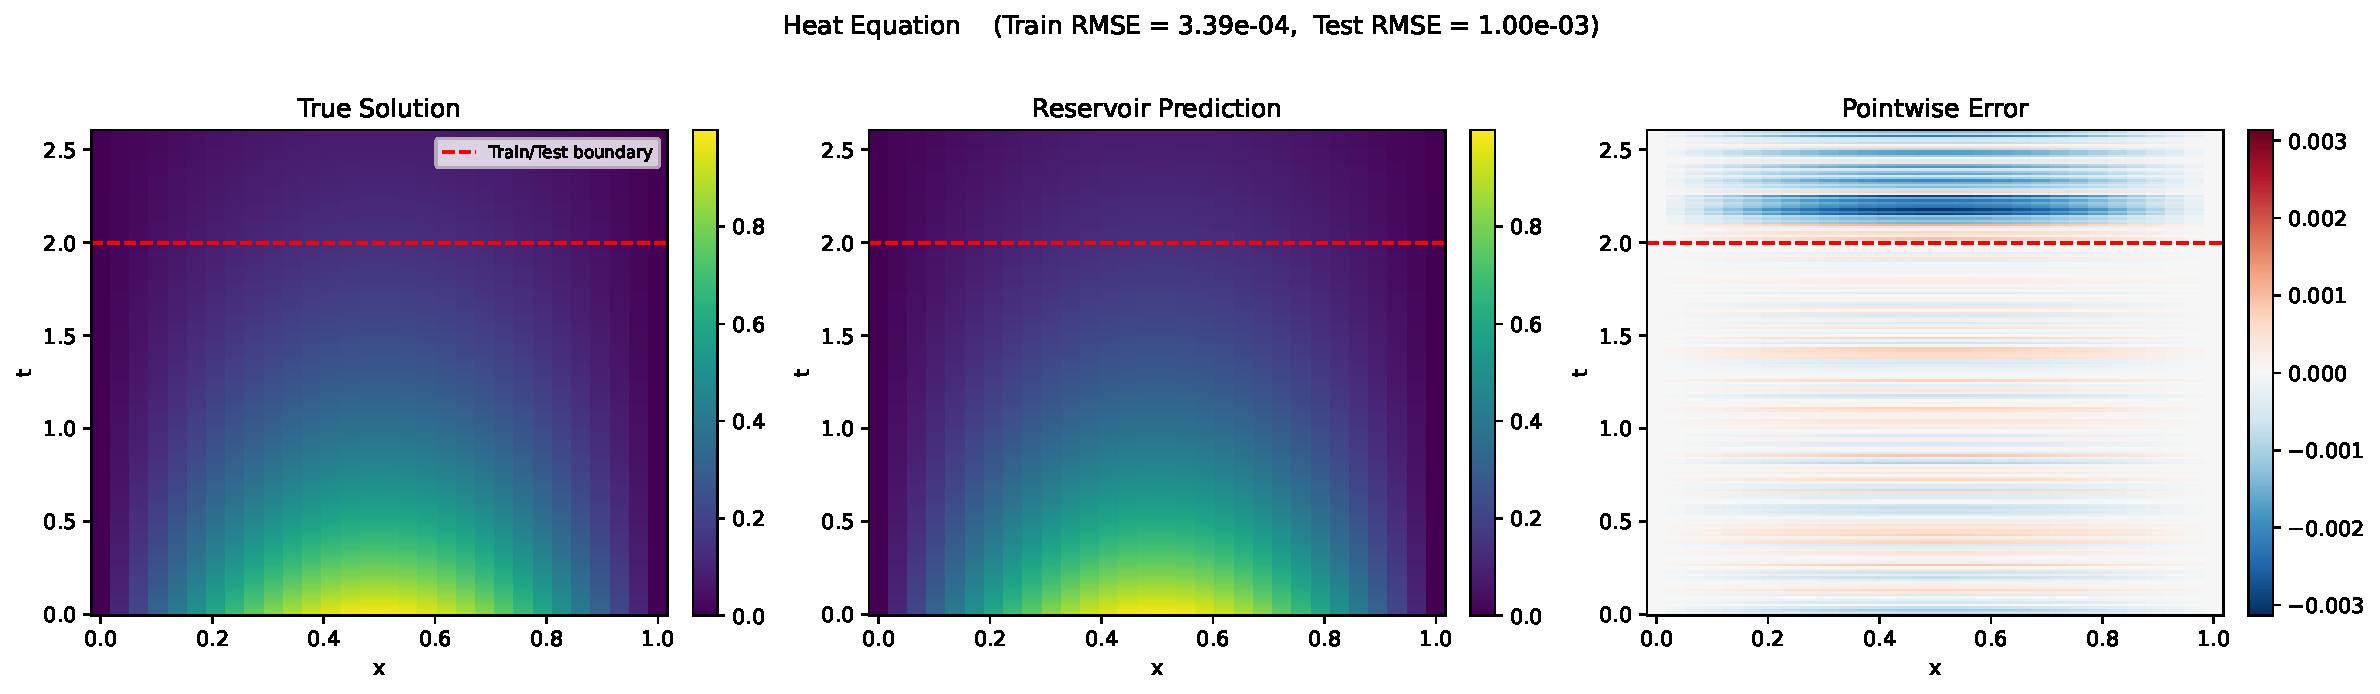
\includegraphics[width=\textwidth]{figures/heat_equation/pde_comparison.pdf}
  \caption{Heat equation ($\alpha=0.1$): true solution (left), reservoir
    prediction (center), and pointwise error (right).  Red dashed line marks
    the train/test boundary.  Multi-subnet 6 high network: train
    RMSE~$= 3.4 \times 10^{-4}$, test RMSE~$= 1.0 \times 10^{-3}$,
    test $R^2 = 0.999$.}
  \label{fig:pde_heat}
\end{figure*}

\subsection{Advection--Diffusion Equation (PDE)}
\label{sec:advdiff}

The advection--diffusion equation introduces a transport term:
\begin{equation}
  \frac{\partial u}{\partial t} = -v\,\frac{\partial u}{\partial x}
    + D\,\frac{\partial^2 u}{\partial x^2},
  \quad x \in [0,1],
\end{equation}
with advection velocity $v = 1.0$, diffusivity $D = 0.01$, and Gaussian
initial condition $u(x,0) = \exp(-50(x-0.3)^2)$.  The solution exhibits
a traveling wave that spreads diffusively while translating---testing the
reservoir's ability to track both spatial translation and dispersive decay.

Figure~\ref{fig:pde_advdiff} shows the reservoir prediction using the
original strongly-coupled network.  The prediction accurately captures
the wavefront propagation and diffusive spreading, with test
$R^2 = 0.954$.  Errors are concentrated at the wavefront where the
spatial gradient is steepest.

\begin{figure*}[t]
  \centering
  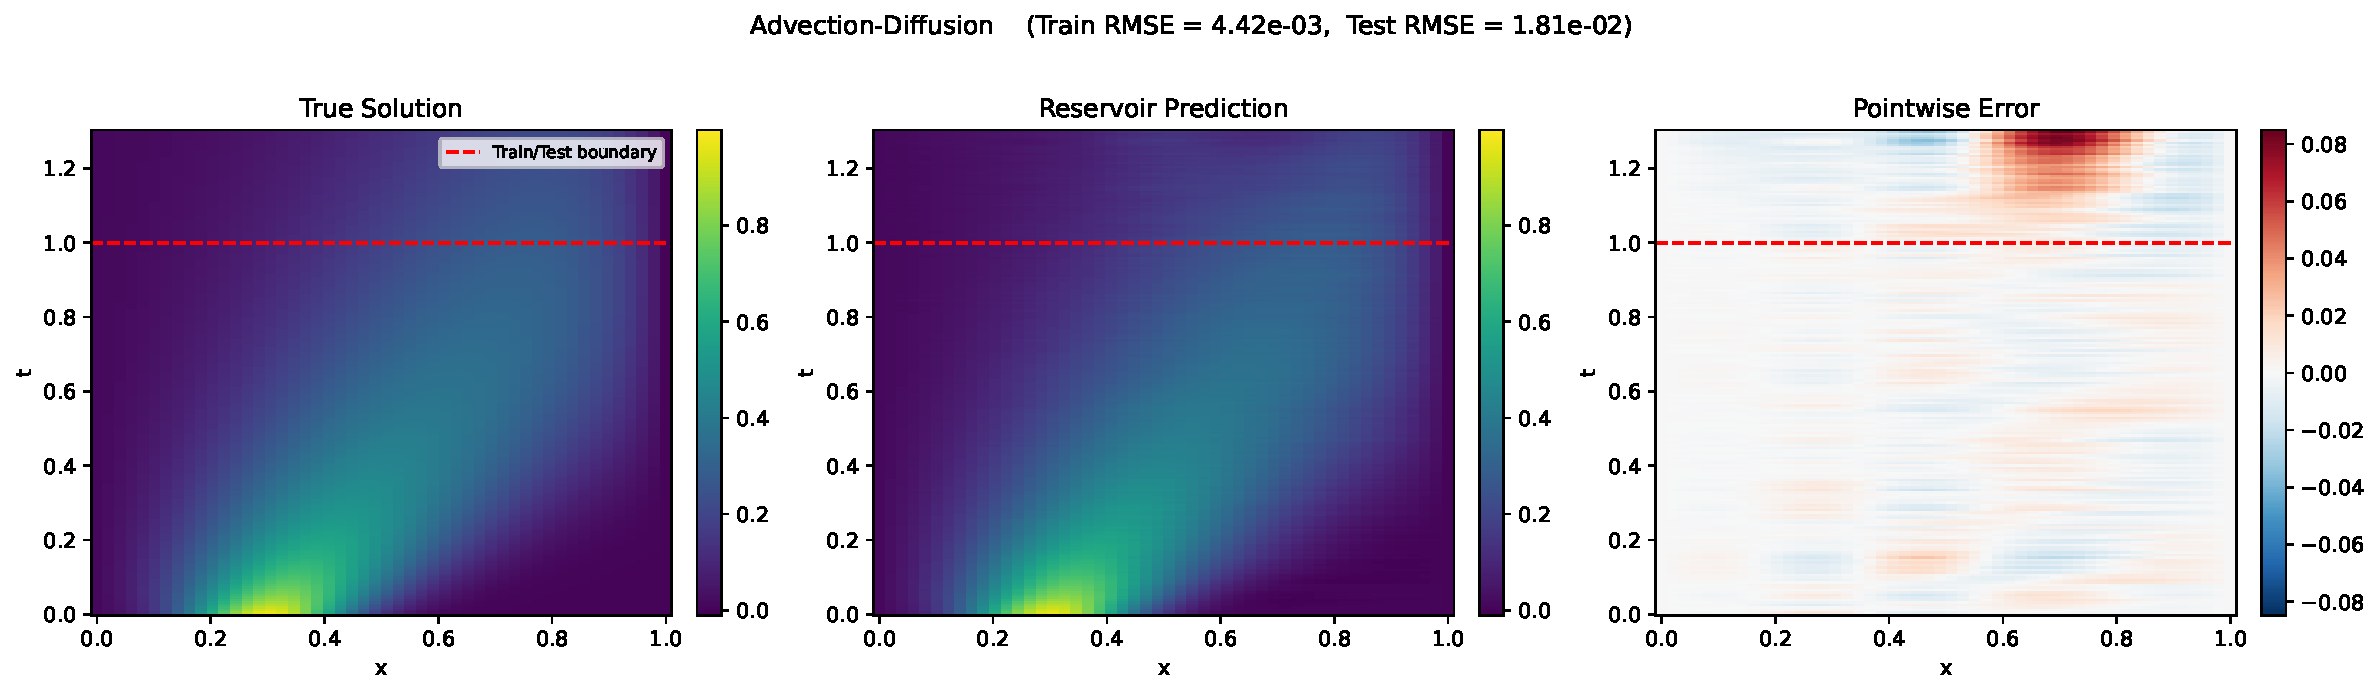
\includegraphics[width=\textwidth]{figures/advection_diffusion/pde_comparison.pdf}
  \caption{Advection--diffusion equation ($v=1$, $D=0.01$): traveling
    Gaussian pulse.  Original network: train RMSE~$= 4.4 \times 10^{-3}$,
    test RMSE~$= 1.8 \times 10^{-2}$, test $R^2 = 0.954$.}
  \label{fig:pde_advdiff}
\end{figure*}

\subsection{Fisher's Equation (PDE)}
\label{sec:fisher}

Fisher's equation adds logistic growth to diffusion:
\begin{equation}
  \frac{\partial u}{\partial t} = D\,\frac{\partial^2 u}{\partial x^2}
    + r\,u(1 - u),
  \quad x \in [0,1],
\end{equation}
with $D = 0.01$ and growth rate $r = 1.0$.  Starting from
$u(x,0) = 0.5\exp(-25(x-0.5)^2)$, the solution develops a traveling
front that connects $u=0$ and $u=1$.  This nonlinear reaction--diffusion
problem tests whether the mass-action reservoir can represent bistable
front propagation.

Figure~\ref{fig:pde_fisher} demonstrates excellent prediction quality
(test $R^2 = 0.994$).  The reservoir captures both the front speed and
the saturation behavior at $u=1$, with only minor errors at the
propagating front interface.

\begin{figure*}[t]
  \centering
  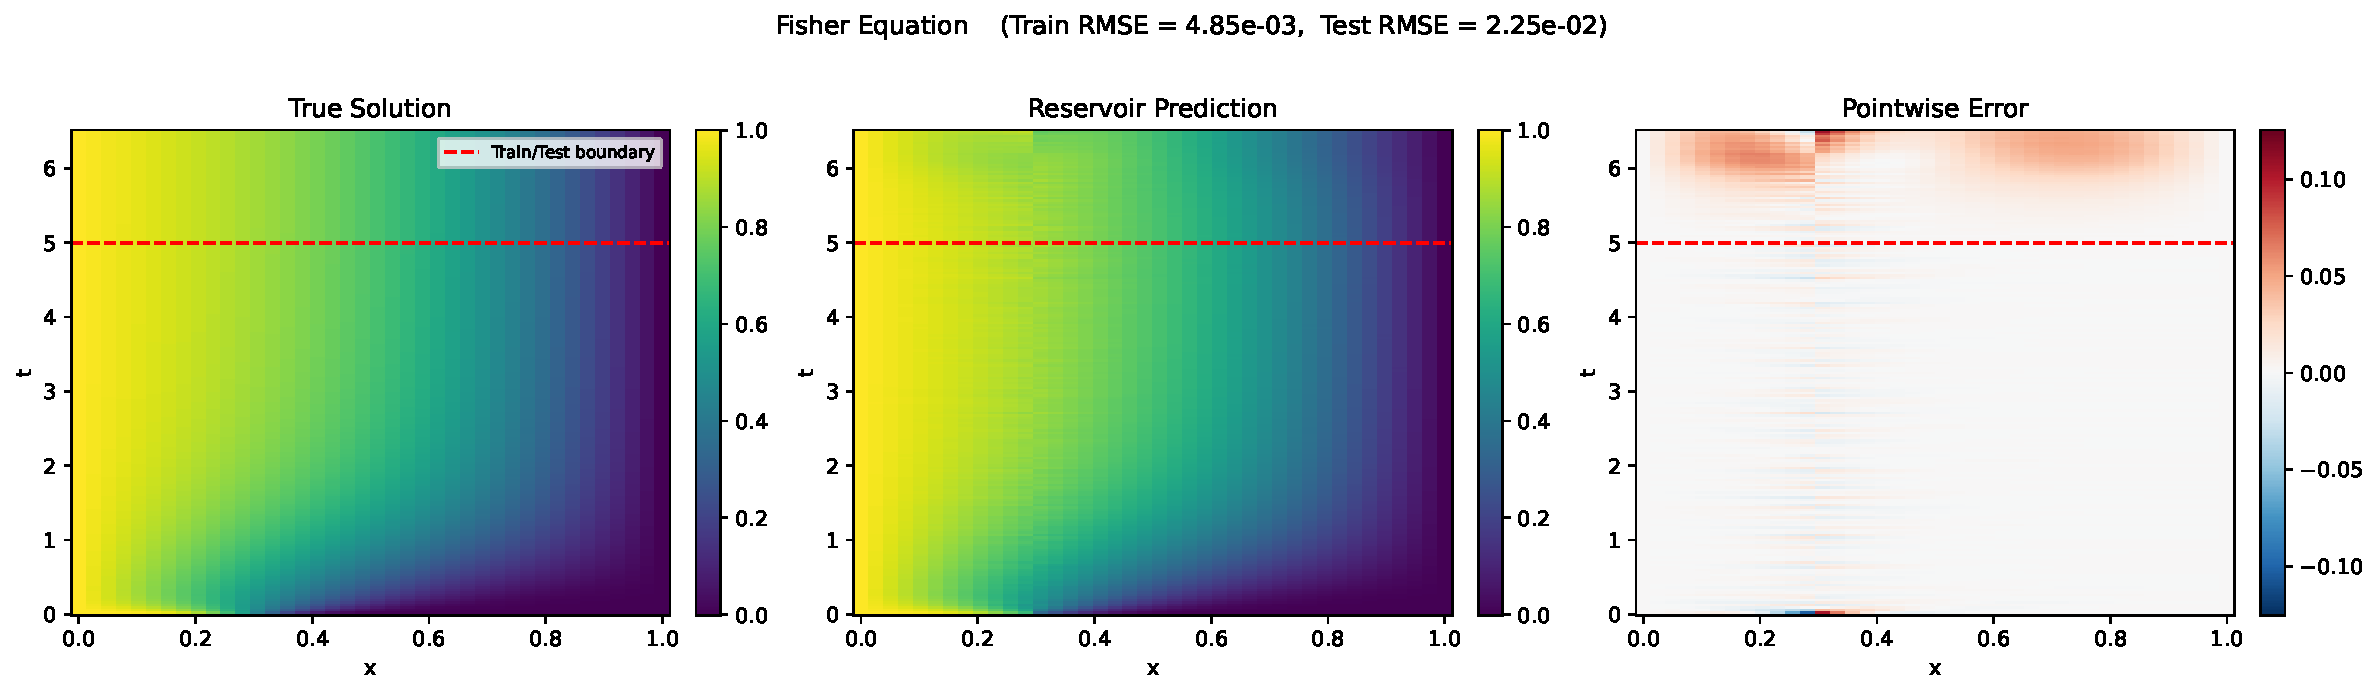
\includegraphics[width=\textwidth]{figures/fisher_equation/pde_comparison.pdf}
  \caption{Fisher's equation ($D=0.01$, $r=1.0$): propagating front.
    Original network: train RMSE~$= 4.8 \times 10^{-3}$,
    test RMSE~$= 2.3 \times 10^{-2}$, test $R^2 = 0.994$.}
  \label{fig:pde_fisher}
\end{figure*}

\subsection{Burgers' Equation (PDE)}
\label{sec:burgers}

Burgers' equation combines nonlinear advection with viscous diffusion:
\begin{equation}
  \frac{\partial u}{\partial t} = -u\frac{\partial u}{\partial x}
    + \nu\frac{\partial^2 u}{\partial x^2},
  \quad x \in [0,1],
\end{equation}
with viscosity $\nu = 0.01$ and initial condition $u(x,0) = \sin(2\pi x)$.
This problem develops steep gradients (shock-like structures) that
challenge any spatial approximation.  The reservoir must capture both the
smooth initial evolution and the subsequent steepening into near-shocks.

Figure~\ref{fig:pde_burgers} shows the reservoir prediction using the
high-complexity multi-subnetwork architecture, which achieves test
$R^2 = 0.983$.  The multi-subnetwork design handles the steep gradients
better than the original network ($R^2 = 0.952$), consistent with the
richer spectral diversity provided by weakly-coupled oscillator modules.

\begin{figure*}[t]
  \centering
  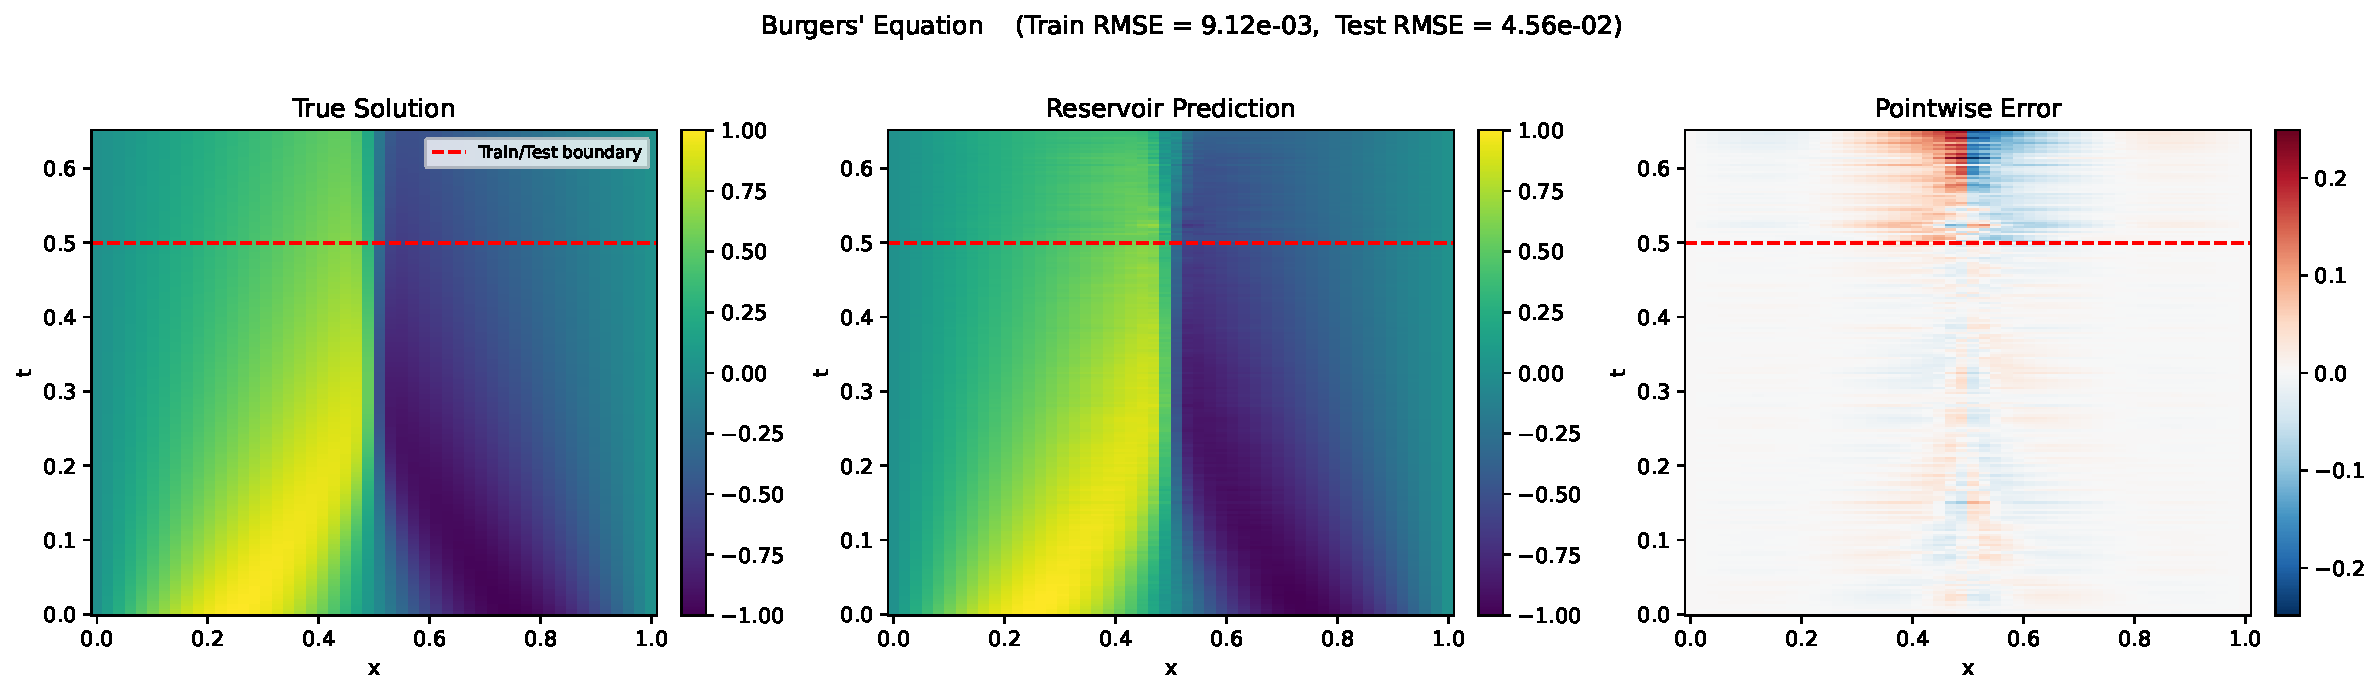
\includegraphics[width=\textwidth]{figures/burgers_equation/pde_comparison.pdf}
  \caption{Burgers' equation ($\nu=0.01$): development of steep gradients.
    Multi-subnet 6 high network: train RMSE~$= 9.1 \times 10^{-3}$,
    test RMSE~$= 4.6 \times 10^{-2}$, test $R^2 = 0.983$.}
  \label{fig:pde_burgers}
\end{figure*}

\subsection{PDE Results Summary}

Table~\ref{tab:pde_summary} summarises the PDE prediction accuracy across
all four benchmarks.  All problems achieve test $R^2 > 0.95$, demonstrating
that the chemical reservoir computing framework generalizes effectively from
ODE to spatiotemporal PDE prediction via the method of lines.  The
high-complexity multi-subnetwork architecture excels on problems with smooth
dynamics (heat equation, $R^2 = 0.999$) and steep spatial features (Burgers,
$R^2 = 0.983$), while the original strongly-coupled network is preferred for
intermediate-complexity problems (advection--diffusion, Fisher).

\begin{table}[t]
\centering
\caption{PDE benchmark summary.  Best network architecture selected per
  problem; $N_{\text{train}}=150$ time steps, $N_{\text{test}}=50$,
  $N_x = 30$ spatial grid points.}
\label{tab:pde_summary}
\small
\begin{tabular}{@{}llccc@{}}
\hline
Problem & Best network & Train RMSE & Test RMSE & Test $R^2$ \\
\hline
Heat equation    & Multi-sub 6 high & $3.4 \times 10^{-4}$ & $1.0 \times 10^{-3}$ & 0.999 \\
Advection--diff. & Original (20 sp) & $4.4 \times 10^{-3}$ & $1.8 \times 10^{-2}$ & 0.954 \\
Fisher equation  & Original (20 sp) & $4.8 \times 10^{-3}$ & $2.3 \times 10^{-2}$ & 0.994 \\
Burgers equation & Multi-sub 6 high & $9.1 \times 10^{-3}$ & $4.6 \times 10^{-2}$ & 0.983 \\
\hline
\end{tabular}
\end{table}

\subsection{Reservoir Dynamics Visualization}

Figure~\ref{fig:trajectories} shows the concentration trajectories of all
20~species in the high-dimensional Brusselator network when driven by the
Van der Pol solution.  The oscillatory dynamics with multiple frequencies
illustrate the rich temporal structure that enables the reservoir to
generalize beyond the training interval.

\begin{figure*}[t]
  \centering
  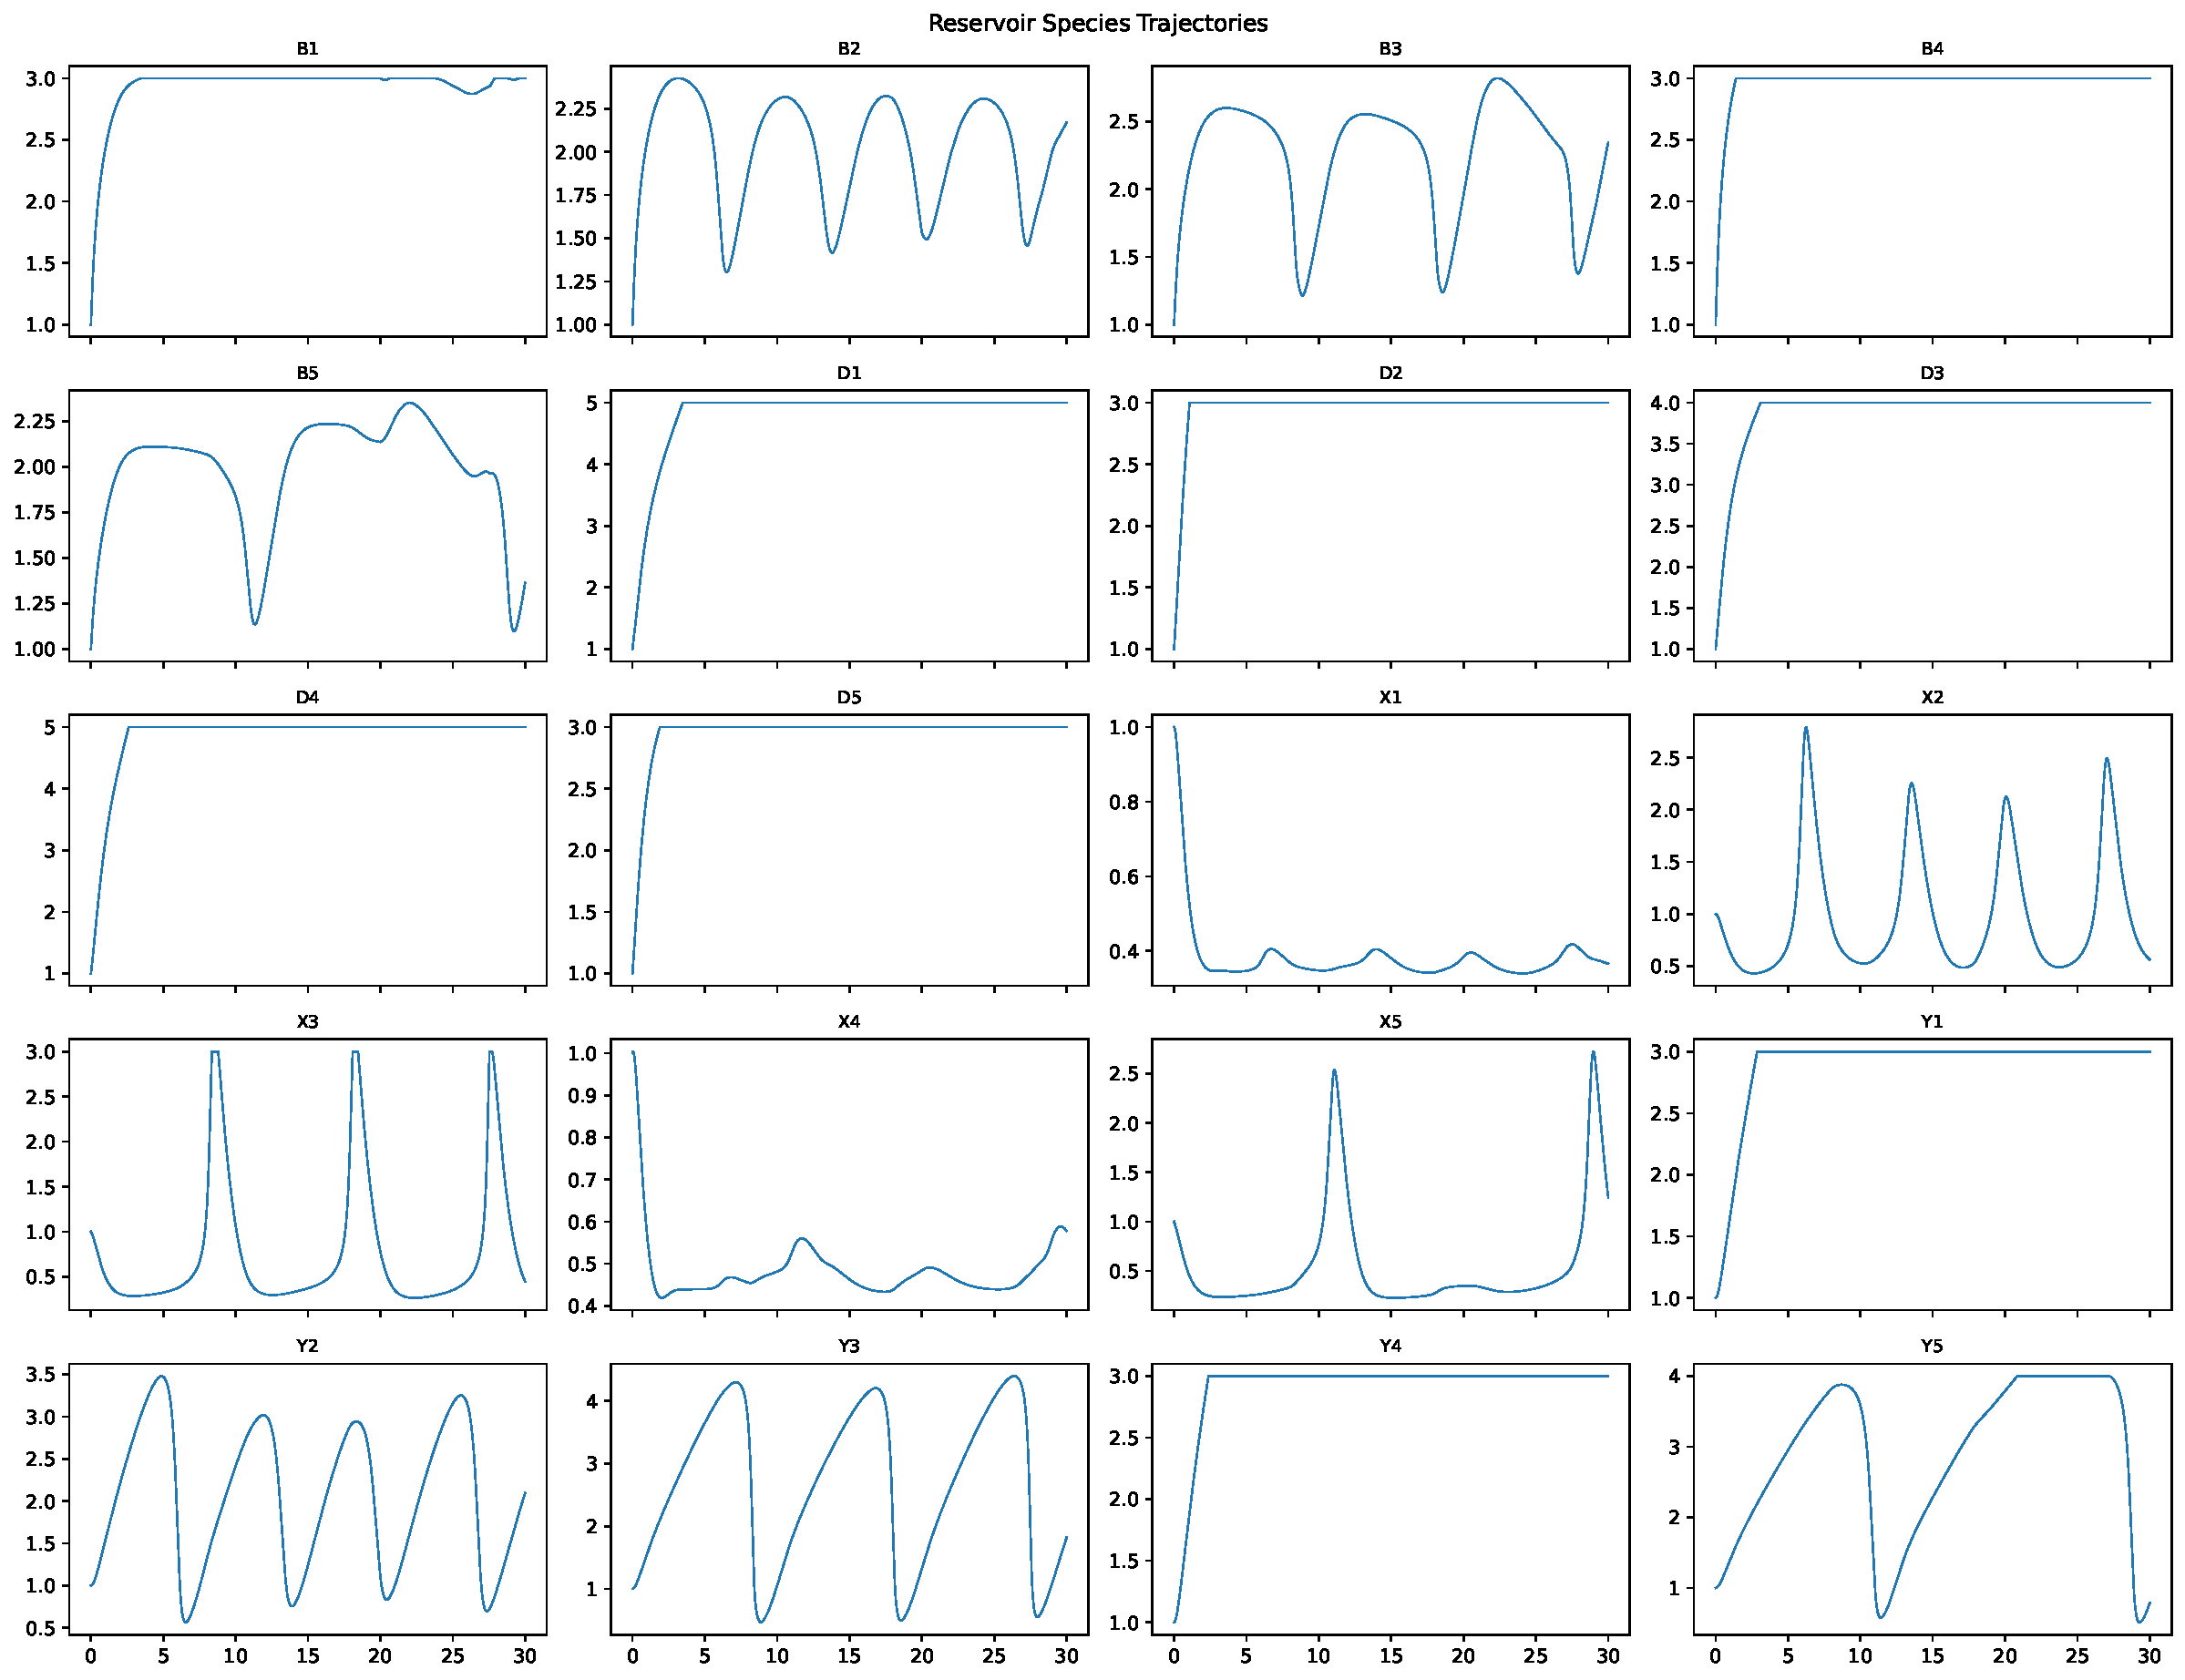
\includegraphics[width=\textwidth]{figures/vanderpol/reservoir_trajectories.pdf}
  \caption{Reservoir species trajectories for the high-dimensional
    Brusselator network driven by the Van der Pol solution.  Each panel
    shows one of the 20 species' concentrations over time.  The limit-cycle
    oscillations at different frequencies provide a diverse feature basis
    for the readout layer.}
  \label{fig:trajectories}
\end{figure*}

\subsection{Network Topology}

The reaction network topology is visualized as a bipartite graph
(Figure~\ref{fig:network}), with species nodes on one side and reaction nodes
on the other.  Edges indicate participation as reactant or product.  This
representation highlights the connectivity structure that determines the
reservoir's dynamical complexity.

\begin{figure*}[t]
  \centering
  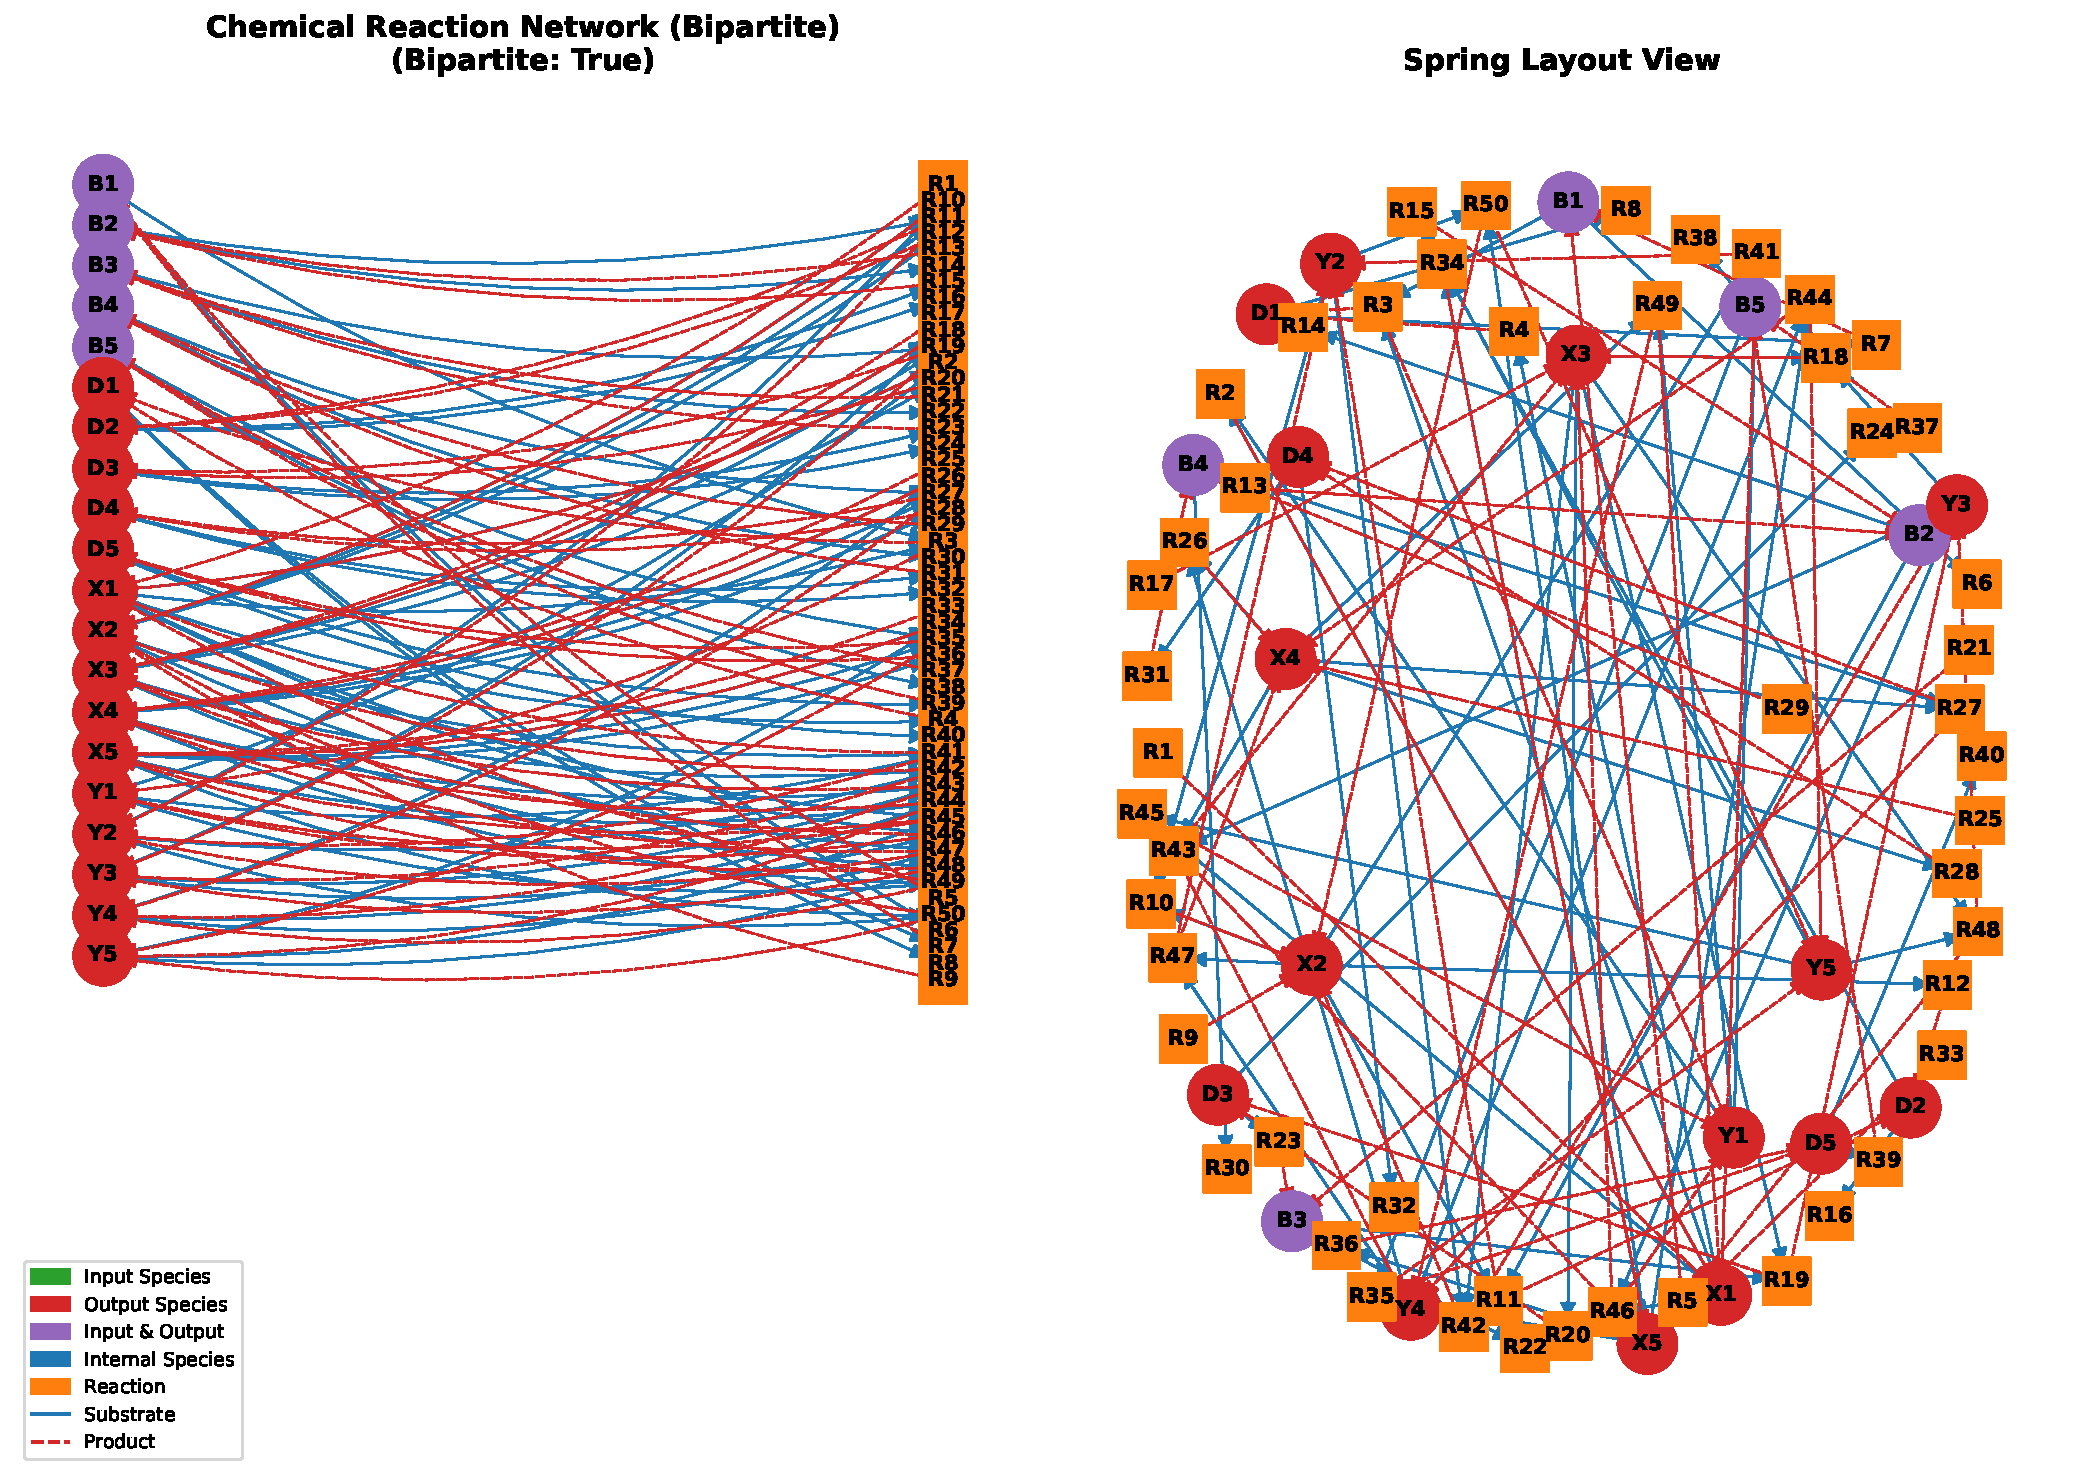
\includegraphics[width=\textwidth]{figures/vanderpol/reaction_network.pdf}
  \caption{Bipartite graph of the high-dimensional Brusselator reaction
    network (20 species, 50 reactions).  Left panel: bipartite layout with
    species (circles) and reaction (squares) nodes.  Right panel: adjacency
    structure.  Green nodes: input species; red nodes: output species;
    purple nodes: species serving as both input and output.}
  \label{fig:network}
\end{figure*}

% ==============================================================================
\section{Performance Metrics}
\label{sec:metrics}

Prediction quality is assessed using multiple complementary metrics:

\begin{itemize}
  \item \textbf{RMSE:}
    $\rmse = \sqrt{N^{-1}\sum_{i}(y_i - \hat{y}_i)^2}$
  \item \textbf{MAE:}
    $\text{MAE} = N^{-1}\sum_i |y_i - \hat{y}_i|$
  \item \textbf{Normalized RMSE:}
    $\text{NRMSE} = \rmse / (\max y - \min y)$
  \item \textbf{Coefficient of determination:}
    $R^2 = 1 - \sum_i(y_i - \hat{y}_i)^2 / \sum_i(y_i - \bar{y})^2$
  \item \textbf{Pearson correlation:} Standard linear correlation $r$
  \item \textbf{Error growth rate:}
    $\lambda$ from exponential fit $e(t) \sim e^{\lambda t}$
  \item \textbf{Prediction stability:}
    $S = 1 - \sigma_e / \bar{e}$
\end{itemize}

For PDE problems, additional spatial diagnostics include the spatial error
distribution $e(x)$ and conservation error (integral deviation between true
and predicted solutions).

\subsection{Open-Loop vs Closed-Loop Comparison}
\label{sec:mode_comparison}

Table~\ref{tab:mode_comparison} summarises the test-region performance of both
prediction modes across the four ODE benchmarks, using the high-dimensional
Brusselator network with delayed feature expansion and $N_{\text{train}}=1600$.

\begin{table}[t]
\centering
\caption{Test $R^2$ for open-loop and closed-loop prediction modes.  The
  feedback scale is $\alpha=0.5$ for closed-loop.  Results vary between runs
  due to stochastic reservoir initialization; representative values are shown.}
\label{tab:mode_comparison}
\small
\begin{tabular}{@{}lcccc@{}}
\hline
Problem & Open-loop $R^2$ & Closed-loop $R^2$ & $N_{\text{test}}$ & Dynamics \\
\hline
Van der Pol     & 0.43  & \textbf{0.64}  & 800 & Limit cycle \\
Brusselator     & 0.51  & \textbf{0.53}  & 800 & Limit cycle \\
Lotka--Volterra & \textbf{0.71}  & 0.61  & 800 & Conservative \\
Lorenz          & $-4.1$ & $\mathbf{-0.3}$  & 400 & Chaotic \\
\hline
\end{tabular}
\end{table}

Several patterns emerge from the comparison:

\begin{itemize}
  \item \textbf{Limit-cycle systems} (Van der Pol, Brusselator) generally
    benefit from closed-loop feedback, which helps maintain phase coherence
    in the test region.  The improvement is most pronounced for the
    Brusselator, where the feedback keeps the prediction locked to the
    oscillation frequency.
  \item \textbf{Conservative systems} (Lotka--Volterra) can be slightly
    degraded by the feedback, which perturbs the energy-conserving structure
    and introduces amplitude drift.  Open-loop is often more reliable for
    such systems.
  \item \textbf{Chaotic systems} (Lorenz) show the most dramatic improvement
    in $R^2$, though both values remain negative, indicating that neither mode
    can outperform a simple mean prediction over the full test horizon.  The
    closed-loop mode extends the useful prediction horizon by approximately
    one Lyapunov time.
  \item \textbf{Computational cost:} open-loop produces test predictions in
    a single forward pass; closed-loop requires $N_{\text{test}}$ sequential
    ODE integrations, increasing wall time by a factor of $\sim\!3$--$5\times$.
\end{itemize}

\subsection{Multi-Subnetwork Architecture}
\label{sec:multisubnet}

To investigate whether reservoir capacity can be improved by network topology,
we introduce a \emph{multi-subnetwork} architecture with three key features:
(i)~multiple weakly-coupled Brusselator oscillator modules connected by small
inter-compartment leakage (diffusive exchange at rate $\sim\!0.005$),
(ii)~sparse skip connections and cross-inhibition between non-adjacent modules,
and (iii)~a shared ``fuel'' species~$F$ with constant feed-in that couples
all modules globally.

\paragraph{Scaling laws.}
Table~\ref{tab:scaling} shows the effect of varying the number of subnetworks
(width) and per-module complexity (depth) on Lorenz prediction.

\begin{table}[t]
\centering
\caption{Network scaling study: Test $R^2$ on the Lorenz system (open-loop,
  $N_{\text{train}}=1600$, $N_{\text{test}}=400$).  Results vary between runs.}
\label{tab:scaling}
\small
\begin{tabular}{@{}llccc@{}}
\hline
Variant & Complexity & Species & Reactions & Lorenz $R^2$ \\
\hline
4 subnets  & standard & 17 & 52  & \textbf{+0.64} \\
6 subnets  & standard & 25 & 78  & +0.57 \\
8 subnets  & standard & 33 & 104 & $-28$ \\
10 subnets & standard & 41 & 130 & $-5.0$ \\
\hline
6 subnets  & minimal  & 25 & 78  & +0.29 \\
6 subnets  & standard & 25 & 78  & +0.43 \\
6 subnets  & high     & 31 & 114 & $-1.2$ \\
\hline
Original (no leakage) & --- & 20 & 50 & $-6.3$ \\
\hline
\end{tabular}
\end{table}

The optimal architecture uses a \emph{small} number of subnetworks (4--6)
with standard complexity.  Increasing width beyond~8 modules degrades
performance, likely because the ridge regression readout cannot resolve
signal from the high-dimensional, weakly-informative feature space without
more training data.  Similarly, adding intermediate species (``high''
complexity) increases the parameter space without proportionally improving
the dynamical repertoire.

\paragraph{Comparison with the original network.}
On the Lorenz system, the multi-subnetwork architecture (4~modules, 17~species)
achieves $R^2 = +0.64$ compared to $R^2 = -6.3$ for the original
strongly-coupled network (20~species).  This dramatic improvement stems from
the weak leakage design: each subnetwork maintains its own distinct oscillation
frequency, providing spectral diversity, while the shared fuel species
introduces a slow global coupling that enriches transient dynamics without
overwhelming the individual modules.

\paragraph{PDE performance.}
Table~\ref{tab:pde_architecture} shows PDE results across architectures.

\begin{table}[t]
\centering
\caption{PDE benchmark: Test $R^2$ for different network architectures.
  All use time-delay features, $N_{\text{train}}=150$ time steps.}
\label{tab:pde_architecture}
\small
\begin{tabular}{@{}lcccc@{}}
\hline
Network & Heat & Advection & Fisher & Burgers \\
\hline
Original (20 sp)       & 0.987 & \textbf{0.957} & \textbf{0.995} & 0.952 \\
Multi-sub 6 std (25 sp) & 0.939 & 0.799 & 0.870 & \textbf{0.968} \\
Multi-sub 6 high (31 sp) & \textbf{0.999} & 0.934 & 0.984 & 0.965 \\
Multi-sub 10 std (41 sp) & 0.988 & 0.909 & 0.961 & 0.963 \\
\hline
\end{tabular}
\end{table}

For PDEs, the high-complexity 6-module network achieves $R^2 = 0.999$ on the
heat equation---the best result across all architectures.  The Burgers equation
(steep gradients) benefits from multi-subnetwork architectures regardless of
complexity.  However, the original strongly-coupled network remains competitive
for smoother PDE problems (advection-diffusion, Fisher equation), where strong
internal oscillation coherence provides an adequate temporal basis.

\paragraph{Design guidelines.}
These results suggest matching the network architecture to the target problem:
\begin{itemize}
  \item \textbf{Chaotic ODE systems:} few (4--6) weakly-coupled subnetworks
    with fuel coupling and leakage provide the best capacity.
  \item \textbf{Periodic ODE systems:} a single strongly-coupled oscillatory
    network (original design) is preferred.
  \item \textbf{Smooth PDEs:} the original or high-complexity multi-subnet
    perform comparably well.
  \item \textbf{PDEs with sharp features:} multi-subnet architectures
    (particularly with higher complexity) capture steep gradients more
    effectively.
\end{itemize}

% ==============================================================================
\section{Discussion}
\label{sec:discussion}

The chemical reservoir computing framework demonstrates several notable
properties:

\paragraph{Role of network topology.}
The choice between a single strongly-coupled network and multiple
weakly-coupled subnetworks with leakage has a dramatic effect on
performance.  For the chaotic Lorenz system, the multi-subnetwork
architecture improves test $R^2$ from $-6.3$ to $+0.64$---a qualitative
shift from failure to useful prediction.  However, periodic systems
prefer the original design, where strong internal coupling produces
coherent oscillations matched to the target dynamics.  This implies
that reservoir ``capacity'' is not simply a function of the number of
species, but depends critically on the \emph{spectral structure} of the
internal dynamics relative to the target system.

\paragraph{Feature expansion matters.}
Quadratic feature expansion dramatically increases the feature dimension
($p(p+3)/2$ features for $p$ species) and can lead to overfitting when
training data are limited.  Time-delay embedding provides a more
parsimonious expansion ($5p$ features) that captures temporal correlations
and generalizes better in practice.

\paragraph{Encoding diversity.}
The multiharmonic encoding provides the richest frequency content for
driving the reservoir, but the mixed encoding offers a good balance of
temporal structure and robustness.

\paragraph{Closed-loop feedback.}
As summarised in Table~\ref{tab:mode_comparison}, the closed-loop mode
substantially improves predictions for limit-cycle systems: the Van~der~Pol
test $R^2$ increases from $0.43$ to $0.64$ because the output feedback
keeps the reservoir synchronized with the oscillation phase.  For the
chaotic Lorenz system, closed-loop prediction improves from $R^2 = -4.1$
to $-0.3$, extending the useful prediction horizon by approximately one
Lyapunov time.  However, the feedback can slightly degrade conservative
systems (Lotka--Volterra), and the optimal feedback scale $\alpha$ is
problem-dependent.  These trade-offs are explored in detail in
Section~\ref{sec:mode_comparison}.

\paragraph{Limitations.}
Even with closed-loop feedback, long-term prediction of chaotic systems
remains fundamentally limited by exponential error growth.  The current
closed-loop implementation feeds predictions back multiplicatively on top
of the encoding signal; a fully autonomous mode (without the encoding
signal during testing) would require richer readout architectures.
The framework also assumes access to the ground-truth solution for
training, positioning it as a learned surrogate model rather than an
\emph{ab initio} solver.  Combining the reservoir with data assimilation
techniques could relax this requirement.

% ==============================================================================
\section{Conclusion}
\label{sec:conclusion}

We have presented \software{}, an open-source Python package for chemical
reservoir computing applied to differential equation solving.  The framework
provides a complete pipeline from reaction network definition through
simulation, feature extraction, and ridge-regression readout, with both
open-loop and closed-loop prediction modes, Bayesian optimization, and
sensitivity analysis for systematic exploration of the design space.  The
closed-loop mode feeds predicted outputs back as reservoir inputs, improving
test-region accuracy for periodic systems and extending the useful prediction
horizon for chaotic systems.

A key finding is that network \emph{topology} strongly determines performance:
a multi-subnetwork architecture with weak inter-compartment leakage and a
shared fuel species achieves $R^2 = +0.64$ on the Lorenz system---a
qualitative improvement over the original strongly-coupled network
($R^2 = -6.3$)---while the original design remains preferable for periodic
problems.  For PDEs, the high-complexity multi-subnetwork variant achieves
$R^2 = 0.999$ on the heat equation.  These results suggest that matching the
network's spectral structure to the target dynamics is as important as
increasing the number of species.

The modular architecture supports user-defined
networks via JSON specification and readily extends to new problem classes.

Future work includes: (i)~fully autonomous closed-loop prediction without
the encoding signal, (ii)~experimental validation with DNA strand
displacement circuits, (iii)~adaptive time-delay selection,
(iv)~multi-fidelity optimization combining low- and high-dimensional
networks, (v)~extension to 2-D and 3-D PDEs via tensor decomposition,
and (vi)~automated topology selection via evolutionary algorithms.

% ==============================================================================
\section*{Acknowledgments}

This work was supported by the Pacific Northwest National Laboratory.
PNNL is operated by Battelle Memorial Institute for the U.S.\ Department
of Energy under Contract DE-AC05-76RL01830.

% ==============================================================================
\section*{Data and Software Availability}

The \software{} package is available at [repository URL] under the
BSD-3-Clause license.  All examples presented in this paper can be reproduced
using the command-line driver:

\begin{verbatim}
python run_reservoir.py \
  --problem vanderpol \
  --network network_configs/high_dimensional_random.json \
  --n-train 1600 --n-test 800 \
  --encoding mixed --features delayed
\end{verbatim}

% ==============================================================================
\bibliographystyle{plain}
% \bibliography{references}

\begin{thebibliography}{10}

\bibitem[Jaeger(2001)]{jaeger2001echo}
H.~Jaeger.
\newblock The ``echo state'' approach to analysing and training recurrent
  neural networks.
\newblock \emph{GMD Report 148}, German National Research Center for
  Information Technology, 2001.

\bibitem[Maass et~al.(2002)]{maass2002real}
W.~Maass, T.~Natschl{\"a}ger, and H.~Markram.
\newblock Real-time computing without stable states: A new framework for
  neural computation based on perturbations.
\newblock \emph{Neural Computation}, 14(11):2531--2560, 2002.

\bibitem[Goudarzi et~al.(2013)]{goudarzi2013dna}
A.~Goudarzi, M.~R. Lakin, and D.~Stefanovic.
\newblock DNA reservoir computing: A novel molecular computing approach.
\newblock In \emph{DNA Computing and Molecular Programming}, pages 76--89.
  Springer, 2013.

\bibitem[Yahiro et~al.(2018)]{yahiro2018reservoir}
W.~Yahiro, N.~Aubert-Kato, and M.~Hagiya.
\newblock Reservoir computing with gene regulatory networks.
\newblock In \emph{Proc.\ Artificial Life Conference}, pages 308--309, 2018.

\bibitem[Takens(1981)]{takens1981detecting}
F.~Takens.
\newblock Detecting strange attractors in turbulence.
\newblock In \emph{Dynamical Systems and Turbulence}, Lecture Notes in
  Mathematics, vol.~898, pages 366--381. Springer, 1981.

\bibitem[Lukoševičius and Jaeger(2009)]{lukosevicius2009reservoir}
M.~Luko{\v{s}}evi{\v{c}}ius and H.~Jaeger.
\newblock Reservoir computing approaches to recurrent neural network training.
\newblock \emph{Computer Science Review}, 3(3):127--149, 2009.

\bibitem[Tanaka et~al.(2019)]{tanaka2019recent}
G.~Tanaka, T.~Yamane, J.~B. H{\'e}roux, R.~Nakane, N.~Kanazawa,
  S.~Takeda, H.~Numata, D.~Nakano, and A.~Hirose.
\newblock Recent advances in physical reservoir computing: A review.
\newblock \emph{Neural Networks}, 115:100--123, 2019.

\bibitem[Nakajima and Fischer(2021)]{nakajima2021reservoir}
K.~Nakajima and I.~Fischer, editors.
\newblock \emph{Reservoir Computing: Theory, Physical Implementations, and
  Applications}.
\newblock Springer, 2021.

\bibitem[Larger et~al.(2012)]{larger2012photonic}
L.~Larger, M.~C. Soriano, D.~Brunner, L.~Appeltant, J.~M. Guti{\'e}rrez,
  L.~Pesquera, C.~R. Mirasso, and I.~Fischer.
\newblock Photonic information processing beyond Turing: An optoelectronic
  implementation of reservoir computing.
\newblock \emph{Optics Express}, 20(3):3241--3249, 2012.

\bibitem[Pathak et~al.(2018)]{pathak2018model}
J.~Pathak, B.~Hunt, M.~Girvan, Z.~Lu, and E.~Ott.
\newblock Model-free prediction of large spatiotemporally chaotic systems from
  data: A reservoir computing approach.
\newblock \emph{Physical Review Letters}, 120(2):024102, 2018.

\end{thebibliography}

\end{document}
